% Options for packages loaded elsewhere
\PassOptionsToPackage{unicode}{hyperref}
\PassOptionsToPackage{hyphens}{url}
\PassOptionsToPackage{dvipsnames,svgnames,x11names}{xcolor}
%
\documentclass[
]{estat/estat}

\usepackage{amsmath,amssymb}
\usepackage{iftex}
\ifPDFTeX
  \usepackage[T1]{fontenc}
  \usepackage[utf8]{inputenc}
  \usepackage{textcomp} % provide euro and other symbols
\else % if luatex or xetex
  \usepackage{unicode-math}
  \defaultfontfeatures{Scale=MatchLowercase}
  \defaultfontfeatures[\rmfamily]{Ligatures=TeX,Scale=1}
\fi
\usepackage{lmodern}
\ifPDFTeX\else  
    % xetex/luatex font selection
    \setmainfont[]{Arial}
\fi
% Use upquote if available, for straight quotes in verbatim environments
\IfFileExists{upquote.sty}{\usepackage{upquote}}{}
\IfFileExists{microtype.sty}{% use microtype if available
  \usepackage[]{microtype}
  \UseMicrotypeSet[protrusion]{basicmath} % disable protrusion for tt fonts
}{}
\makeatletter
\@ifundefined{KOMAClassName}{% if non-KOMA class
  \IfFileExists{parskip.sty}{%
    \usepackage{parskip}
  }{% else
    \setlength{\parindent}{0pt}
    \setlength{\parskip}{6pt plus 2pt minus 1pt}}
}{% if KOMA class
  \KOMAoptions{parskip=half}}
\makeatother
\usepackage{xcolor}
\usepackage[left=3cm,right=2cm,top=3cm,bottom=2cm]{geometry}
\setlength{\emergencystretch}{3em} % prevent overfull lines
\setcounter{secnumdepth}{5}
% Make \paragraph and \subparagraph free-standing
\makeatletter
\ifx\paragraph\undefined\else
  \let\oldparagraph\paragraph
  \renewcommand{\paragraph}{
    \@ifstar
      \xxxParagraphStar
      \xxxParagraphNoStar
  }
  \newcommand{\xxxParagraphStar}[1]{\oldparagraph*{#1}\mbox{}}
  \newcommand{\xxxParagraphNoStar}[1]{\oldparagraph{#1}\mbox{}}
\fi
\ifx\subparagraph\undefined\else
  \let\oldsubparagraph\subparagraph
  \renewcommand{\subparagraph}{
    \@ifstar
      \xxxSubParagraphStar
      \xxxSubParagraphNoStar
  }
  \newcommand{\xxxSubParagraphStar}[1]{\oldsubparagraph*{#1}\mbox{}}
  \newcommand{\xxxSubParagraphNoStar}[1]{\oldsubparagraph{#1}\mbox{}}
\fi
\makeatother


\providecommand{\tightlist}{%
  \setlength{\itemsep}{0pt}\setlength{\parskip}{0pt}}\usepackage{longtable,booktabs,array}
\usepackage{calc} % for calculating minipage widths
% Correct order of tables after \paragraph or \subparagraph
\usepackage{etoolbox}
\makeatletter
\patchcmd\longtable{\par}{\if@noskipsec\mbox{}\fi\par}{}{}
\makeatother
% Allow footnotes in longtable head/foot
\IfFileExists{footnotehyper.sty}{\usepackage{footnotehyper}}{\usepackage{footnote}}
\makesavenoteenv{longtable}
\usepackage{graphicx}
\makeatletter
\def\maxwidth{\ifdim\Gin@nat@width>\linewidth\linewidth\else\Gin@nat@width\fi}
\def\maxheight{\ifdim\Gin@nat@height>\textheight\textheight\else\Gin@nat@height\fi}
\makeatother
% Scale images if necessary, so that they will not overflow the page
% margins by default, and it is still possible to overwrite the defaults
% using explicit options in \includegraphics[width, height, ...]{}
\setkeys{Gin}{width=\maxwidth,height=\maxheight,keepaspectratio}
% Set default figure placement to htbp
\makeatletter
\def\fps@figure{htbp}
\makeatother

\authors{%
    Tales Vaz
    
}

% escreva o nome do cliente aqui
% se for mais de um separe por \\
\client{%
    João Neves
}
% Baixando pacotes
\RequirePackage{fancyhdr}
\RequirePackage{graphicx}

\setlength\headheight{28pt}  

\setlength{\parindent}{15pt} % Adiciona indentação nos parágrafos
\setlength{\parskip}{0pt} % Adiciona 0 espaço entro os parágrafos

\newcommand{\estat}{\textbf{ESTAT}\xspace}
\newcommand{\direx}{\textbf{DIREX}\xspace}
\makeatletter
\@ifpackageloaded{caption}{}{\usepackage{caption}}
\AtBeginDocument{%
\ifdefined\contentsname
  \renewcommand*\contentsname{Índice}
\else
  \newcommand\contentsname{Índice}
\fi
\ifdefined\listfigurename
  \renewcommand*\listfigurename{Lista de Figuras}
\else
  \newcommand\listfigurename{Lista de Figuras}
\fi
\ifdefined\listtablename
  \renewcommand*\listtablename{Lista de Tabelas}
\else
  \newcommand\listtablename{Lista de Tabelas}
\fi
\ifdefined\figurename
  \renewcommand*\figurename{Figura}
\else
  \newcommand\figurename{Figura}
\fi
\ifdefined\tablename
  \renewcommand*\tablename{Tabela}
\else
  \newcommand\tablename{Tabela}
\fi
}
\@ifpackageloaded{float}{}{\usepackage{float}}
\floatstyle{ruled}
\@ifundefined{c@chapter}{\newfloat{codelisting}{h}{lop}}{\newfloat{codelisting}{h}{lop}[chapter]}
\floatname{codelisting}{Listagem}
\newcommand*\listoflistings{\listof{codelisting}{Lista de Listagens}}
\captionsetup{labelsep=colon}
\makeatother
\makeatletter
\makeatother
\makeatletter
\@ifpackageloaded{caption}{}{\usepackage{caption}}
\@ifpackageloaded{subcaption}{}{\usepackage{subcaption}}
\makeatother

\ifLuaTeX
\usepackage[bidi=basic]{babel}
\else
\usepackage[bidi=default]{babel}
\fi
\babelprovide[main,import]{portuguese}
\ifPDFTeX
\else
\babelfont{rm}[]{Arial}
\fi
% get rid of language-specific shorthands (see #6817):
\let\LanguageShortHands\languageshorthands
\def\languageshorthands#1{}
\ifLuaTeX
  \usepackage{selnolig}  % disable illegal ligatures
\fi
\usepackage{bookmark}

\IfFileExists{xurl.sty}{\usepackage{xurl}}{} % add URL line breaks if available
\urlstyle{same} % disable monospaced font for URLs
\hypersetup{
  pdftitle={Referencial Teórico},
  pdflang={pt},
  colorlinks=true,
  linkcolor={black},
  filecolor={black},
  citecolor={black},
  urlcolor={black},
  pdfcreator={LaTeX via pandoc}}


\title{Referencial Teórico}
\author{}
\date{}

\begin{document}
\maketitle

% Limpando tudo
\fancyhf{} 

% Ajustes do header
\fancyhead[L]{} % limpando o lado esquerdo
\fancyhead[R]{
\includegraphics[width=0.20\textwidth]{estat/imagens/estat.png}} % adicionando logo no canto direito
\renewcommand{\headrulewidth}{0pt}   % sem linha embaixo da logo

% Ajustes de fim de página
\fancyfoot[R]{\textcolor{white}{\thepage}} % Número em branco no canto direito

% Aplicando o estilo que acabamos de criar
\pagestyle{fancy} 

\renewcommand*\contentsname{Sumário}
{
\hypersetup{linkcolor=}
\setcounter{tocdepth}{3}
\tableofcontents
}

\section{Análise Descritiva
Univariada}\label{anuxe1lise-descritiva-univariada}

\subsection{Frequência Relativa}\label{frequuxeancia-relativa}

A frequência relativa é utilizada para a comparação entre classes de uma
variável categórica com \(c\) categorias, ou para comparar uma mesma
categoria em diferentes estudos.

A frequência relativa da categoria \(j\) é dada por:

\[
f_j=\frac{n_j}{n}
\]

Com:

\begin{itemize}
\item
  \(j = 1, \, ..., \, c\)
\item
  \(n_j =\) número de observações da categoria \(j\)
\item
  \(n =\) número total de observações
\end{itemize}

Geralmente, a frequência relativa é utilizada em porcentagem, dada por:

\[100 \times f_j\]

\subsection{Média}\label{muxe9dia}

A média é a soma das observações dividida pelo número total delas, dada
pela fórmula:

\[\bar{X}=\frac{\sum\limits_{i=1}^{n}X_i}{n}\]

Com:

\begin{itemize}
\item
  \(i = 1, \, 2, \, ..., \, n\)
\item
  \(n =\) número total de observações
\end{itemize}

\subsection{Mediana}\label{mediana}

Sejam as \(n\) observações de um conjunto de dados
\(X=X_{(1)},X_{(2)},\ldots, X_{(n)}\) de determinada variável ordenadas
de forma crescente. A mediana do conjunto de dados \(X\) é o valor que
deixa metade das observações abaixo dela e metade dos dados acima.

Com isso, pode-se calcular a mediana da seguinte forma:

\[
med(X) =
    \begin{cases}
         X_{\frac{n+1}{2}}, \textrm{para n ímpar} \\
         \frac{X_{\frac{n}{2}}+X_{\frac{n}{2} + 1}}{2}, \textrm{para n par} \\
    \end{cases}
\]

\subsection{Quartis}\label{quartis}

Os quartis são separatrizes que dividem o conjunto de dados em quatro
partes iguais. O primeiro quartil (ou inferior) delimita os 25\% menores
valores, o segundo representa a mediana, e o terceiro delimita os 25\%
maiores valores. Inicialmente deve-se calcular a posição do quartil:

\begin{itemize}
\item
  Posição do primeiro quartil \(P_1\): \[P_1=\frac{n+1}{4}\]
\item
  Posição da mediana (segundo quartil) \(P_2\): \[P_2 = \frac{n+1}{2}\]
\item
  Posição do terceiro quartil \(P_3\): \[P_3=\frac{3 \times (n+1)}{4}\]
\end{itemize}

Com \(n\) sendo o tamanho da amostra. Dessa forma,
\(X_{\left( P_i \right)}\) é o valor do \(i\)-ésimo quartil, onde
\(X_{\left( j \right)}\) representa a \(j\)-ésima observação dos dados
ordenados.

Se o cálculo da posição resultar em uma fração, deve-se fazer a média
entre o valor que está na posição do inteiro anterior e do seguinte ao
da posição.

\subsection{Variância}\label{variuxe2ncia}

A variância é uma medida que avalia o quanto os dados estão dispersos em
relação à média, em uma escala ao quadrado da escala dos dados.

\subsubsection{Variância Populacional}\label{variuxe2ncia-populacional}

Para uma população, a variância é dada por:

\[\sigma^2=\frac{\sum\limits_{i=1}^{N}\left(X_i - \mu\right)^2}{N}\]

Com:

\begin{itemize}
\item
  \(X_i =\) \(i\)-ésima observação da população
\item
  \(\mu =\) média populacional
\item
  \(N =\) tamanho da população
\end{itemize}

\subsubsection{Variância Amostral}\label{variuxe2ncia-amostral}

Para uma amostra, a variância é dada por:

\[S^2=\frac{\sum\limits_{i=1}^{n}\left(X_i - \bar{X}\right)^2}{n-1}\]

Com:

\begin{itemize}
\item
  \(X_i =\) i-ésima observação da amostra
\item
  \(\bar{X} =\) média amostral
\item
  \(n =\) tamanho da amostra
\end{itemize}

\subsection{Desvio Padrão}\label{desvio-padruxe3o}

O desvio padrão é a raiz quadrada da variância. Ele avalia o quanto os
dados estão dispersos em relação à média.

\subsubsection{Desvio Padrão
Populacional}\label{desvio-padruxe3o-populacional}

Para uma população, o desvio padrão é dado por:

\[\sigma=\sqrt{\frac{\sum\limits_{i=1}^{N}\left(X_i - \mu\right)^2}{N}}\]

Com:

\begin{itemize}
\item
  \(X_i =\) i-ésima observação da população
\item
  \(\mu =\) média populacional
\item
  \(N =\) tamanho da população
\end{itemize}

\subsubsection{Desvio Padrão Amostral}\label{desvio-padruxe3o-amostral}

Para uma amostra, o desvio padrão é dado por:

\[S=\sqrt{\frac{\sum\limits_{i=1}^{n}\left(X_i - \bar{X}\right)^2}{n-1}}\]

Com:

\begin{itemize}
\item
  \(X_i =\) i-ésima observação da amostra
\item
  \(\bar{X} =\) média amostral
\item
  \(n =\) tamanho da amostra
\end{itemize}

\subsection{Coeficiente de
Variação}\label{coeficiente-de-variauxe7uxe3o}

O coeficiente de variação fornece a dispersão dos dados em relação à
média. Quanto menor for o seu valor, mais homogêneos serão os dados. O
coeficiente de variação é considerado baixo (apontando um conjunto de
dados homogêneo) quando for menor ou igual a 25\%. Ele é dado pela
fórmula:

\[C_V=\frac{S}{\bar{X}}\times 100\]

Com:

\begin{itemize}
\item
  \(S =\) desvio padrão amostral
\item
  \(\bar{X} =\) média amostral
\end{itemize}

\subsection{Coeficiente de Assimetria}\label{coeficiente-de-assimetria}

O coeficiente de assimetria quantifica a simetria dos dados. Um valor
positivo indica que os dados estão concentrados à esquerda em sua função
de distribuição, enquanto um valor negativo indica maior concentração à
direita. A fórmula é:

\[C_{Assimetria} = \frac{1}{n}\times\sum\limits_{i=1}^{n} \left(\frac{X_i - \bar{X}}{S}\right)^3 \]

Com:

\begin{itemize}
\item
  \(X_i =\) i-ésima observação da amostra
\item
  \(\bar{X} =\) média amostral
\item
  \(S=\) desvio padrão amostral
\item
  \(n=\) tamanho da amostra
\end{itemize}

\subsection{Curtose}\label{curtose}

O coeficiente de curtose quantifica o achatamento da função de
distribuição em relação à distribuição Normal e é dado por:

\[Curtose = \frac{1}{n}\times\sum\limits_{i=1}^{n}\left(\frac{ X_i-\bar{X} }{S} \right)^4 - 3\]

Com:

\begin{itemize}
\item
  \(X_i =\) i-ésima observação da amostra
\item
  \(\bar{X} =\) média amostral
\item
  \(S =\) desvio padrão amostral
\item
  \(n =\) tamanho da amostra
\end{itemize}

Uma distribuição é dita mesocúrtica quando possui curtose nula. Quando a
curtose é positiva, a distribuição é leptocúrtica (mais afunilada e com
pico). Valores negativos indicam uma distribuição platicúrtica (mais
achatada).

\subsection{Boxplot}\label{boxplot}

O boxplot é uma representação gráfica na qual se pode perceber de forma
mais clara como os dados estão distribuídos. A figura abaixo ilustra um
exemplo de boxplot.

\begin{figure}[H]

\caption{Exemplo de boxplot}

{\centering 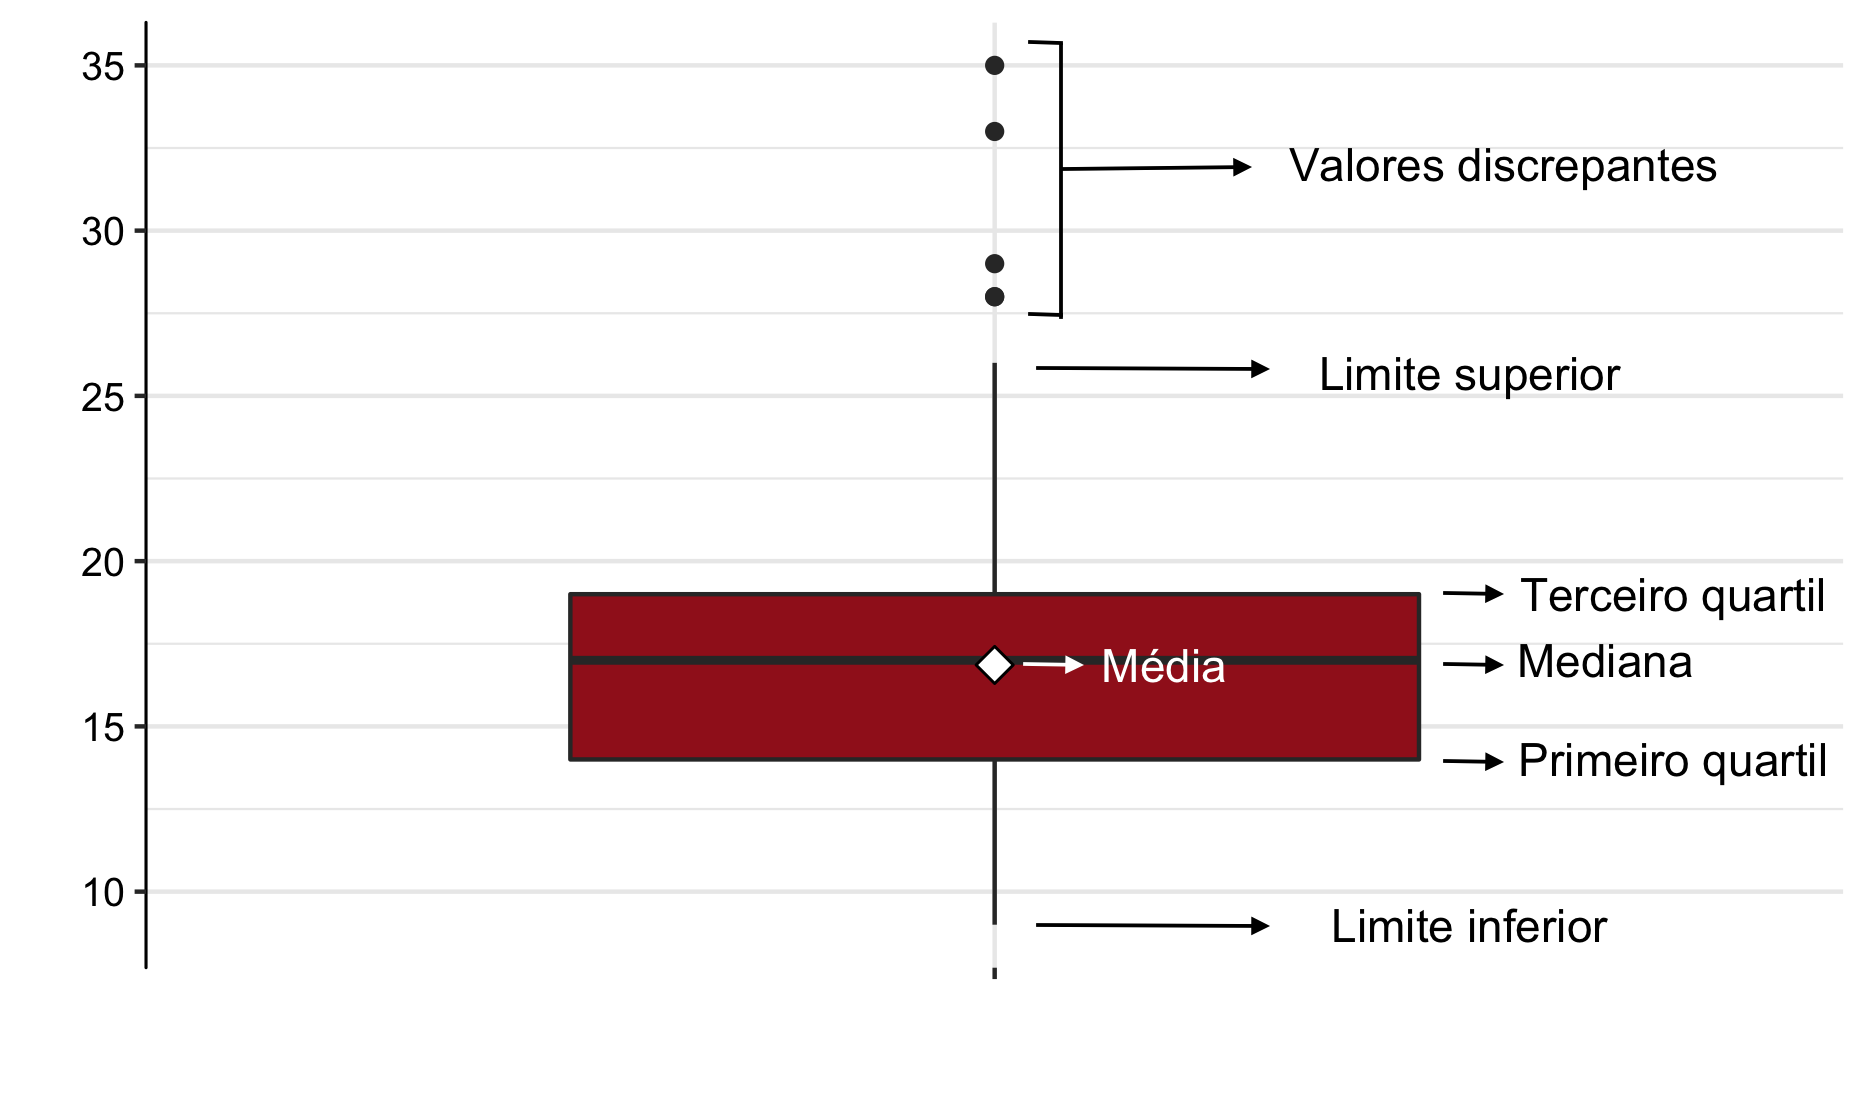
\includegraphics{images/box_uni.png}

}

\end{figure}%

A porção inferior do retângulo diz respeito ao primeiro quartil,
enquanto a superior indica o terceiro quartil. Já o traço no interior do
retângulo representa a mediana do conjunto de dados, ou seja, o valor em
que o conjunto de dados é dividido em dois subconjuntos de mesmo
tamanho. A média é representada pelo losango branco e os pontos são
\emph{outliers}. Os \emph{outliers} são valores discrepantes da série de
dados, ou seja, valores que não demonstram a realidade de um conjunto de
dados.

\subsection{Histograma}\label{histograma}

O histograma é uma representação gráfica utilizada para a visualização
da distribuição dos dados e pode ser construído por valores absolutos,
frequência relativa ou densidade. A figura abaixo ilustra um exemplo de
histograma.

\begin{figure}[H]

\caption{Exemplo de histograma}

{\centering 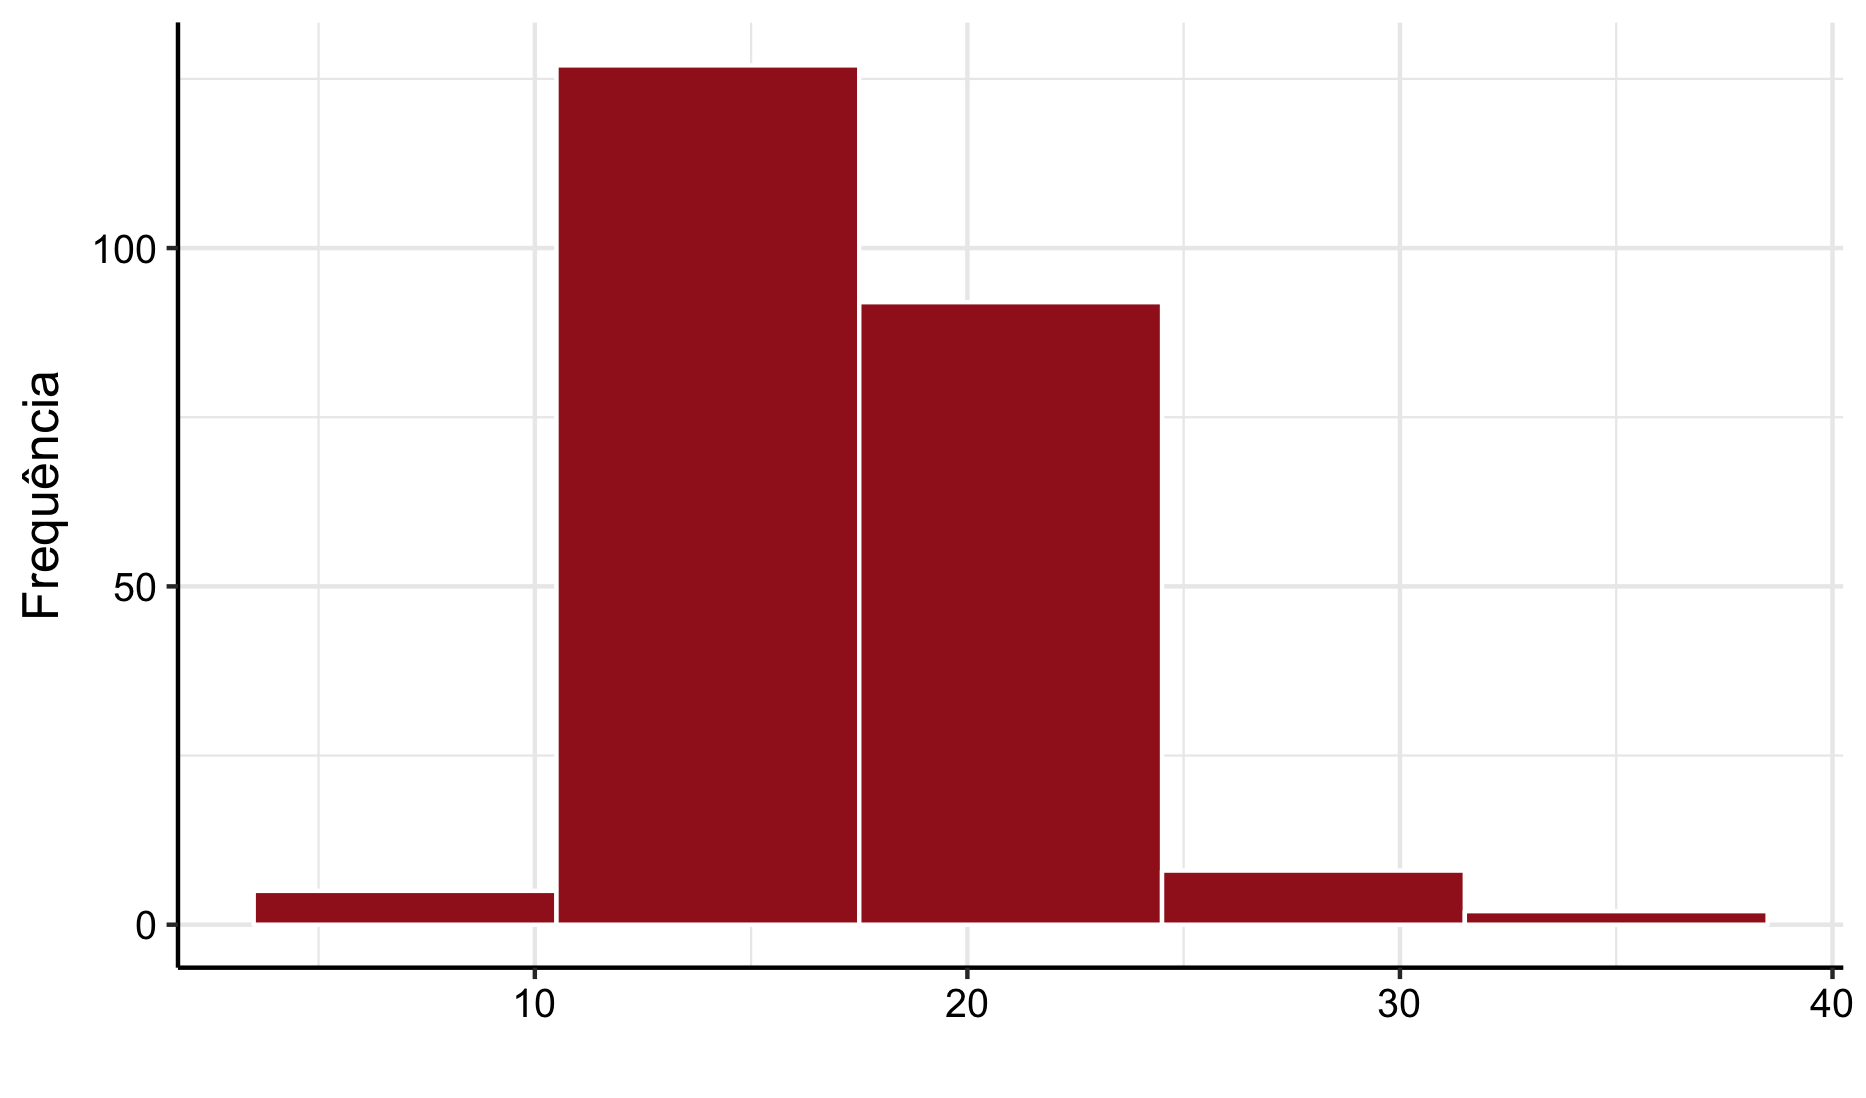
\includegraphics{images/hist_uni.png}

}

\end{figure}%

\subsection{Gráfico de Dispersão}\label{gruxe1fico-de-dispersuxe3o}

O gráfico de dispersão é uma representação gráfica utilizada para
ilustrar o comportamento conjunto de duas variáveis quantitativas. A
figura abaixo ilustra um exemplo de gráfico de dispersão, onde cada
ponto representa uma observação do banco de dados.

\begin{figure}[H]

\caption{Exemplo de Gráfico de Dispersão}

{\centering 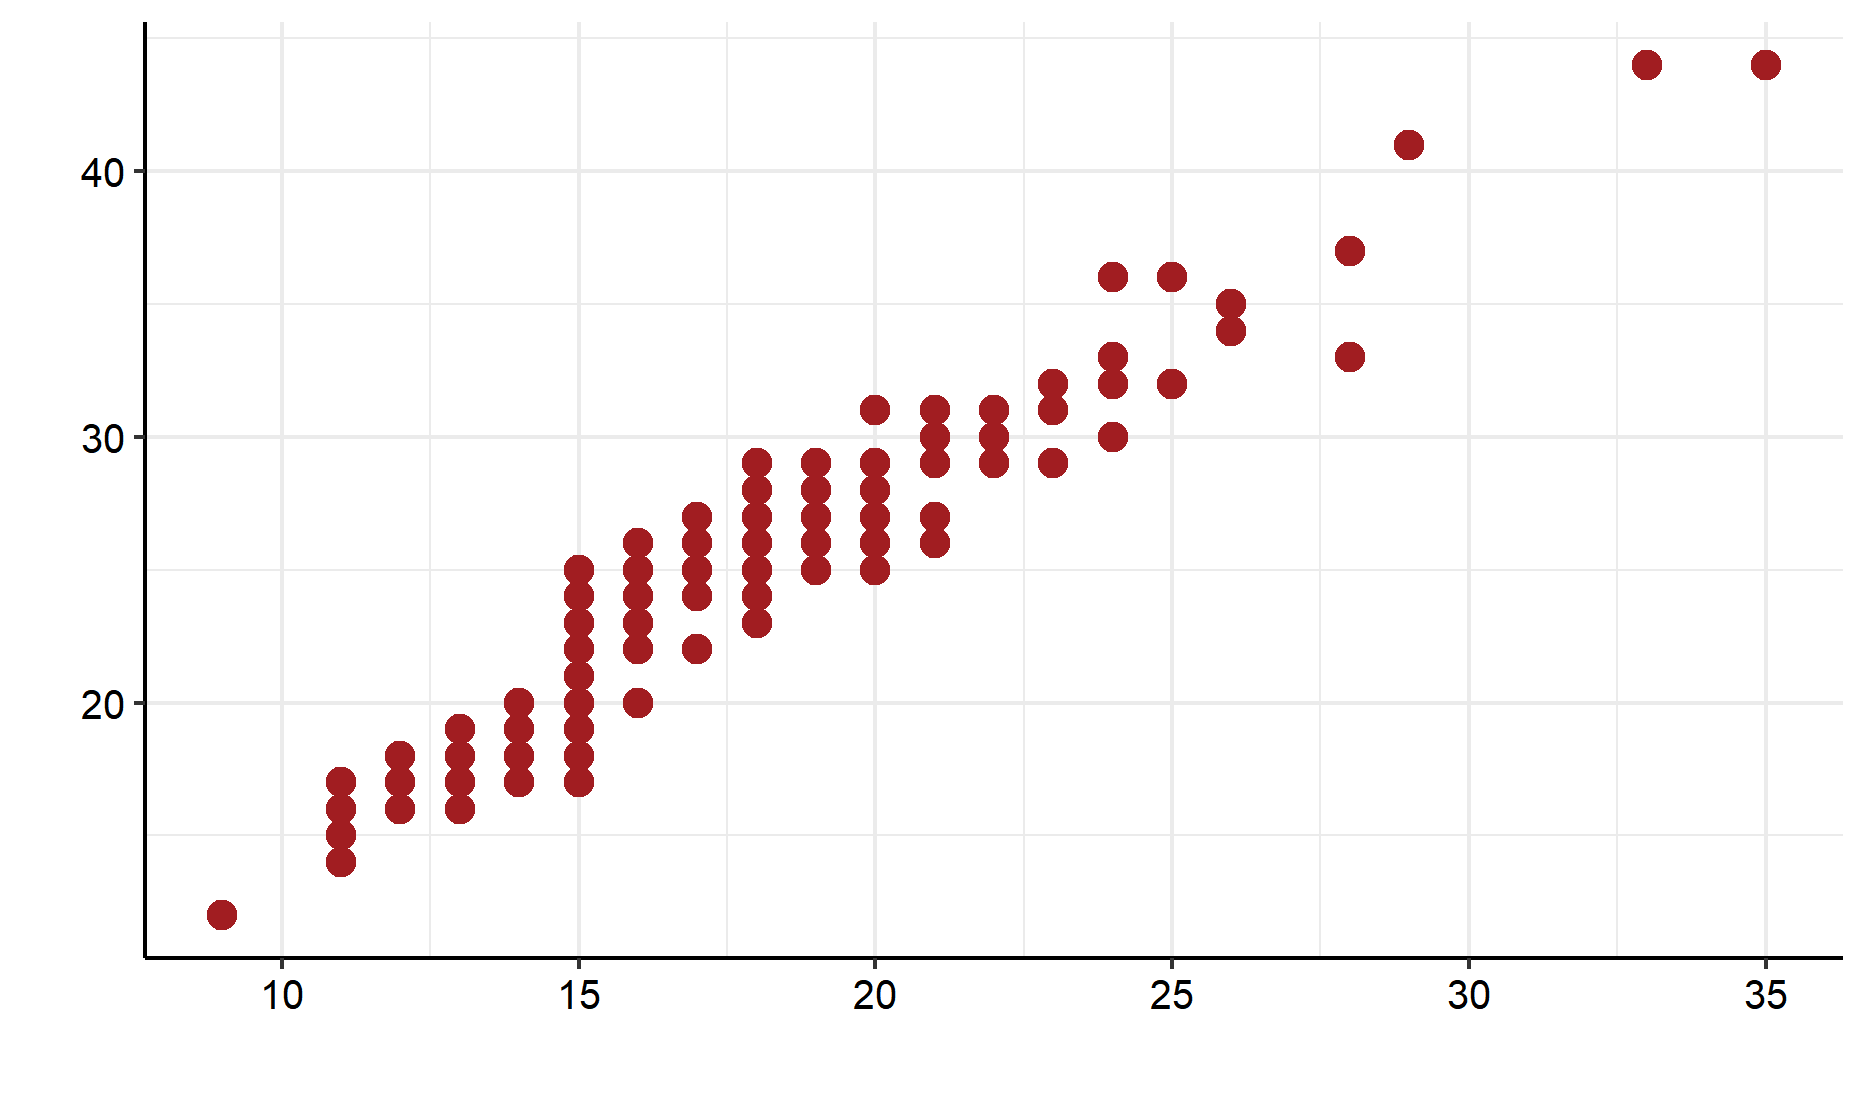
\includegraphics{images/disp_uni.png}

}

\end{figure}%

\subsection{Tipos de Variáveis}\label{tipos-de-variuxe1veis}

\subsubsection{Qualitativas}\label{qualitativas}

As variáveis qualitativas são as variáveis não numéricas, que
representam categorias ou características da população. Estas
subdividem-se em:

\begin{itemize}
\tightlist
\item
  \textbf{Nominais}: quando não existe uma ordem entre as categorias da
  variável (exemplos: sexo, cor dos olhos, fumante ou não, etc)
\item
  \textbf{Ordinais}: quando existe uma ordem entre as categorias da
  variável (exemplos: nível de escolaridade, mês, estágio de doença,
  etc)
\end{itemize}

\subsubsection{Quantitativas}\label{quantitativas}

As variáveis quantitativas são as variáveis numéricas, que representam
características numéricas da população, ou seja, quantidades. Estas
subdividem-se em:

\begin{itemize}
\tightlist
\item
  \textbf{Discretas}: quando os possíveis valores são enumeráveis
  (exemplos: número de filhos, número de cigarros fumados, etc)
\item
  \textbf{Contínuas}: quando os possíveis valores são resultado de
  medições (exemplos: massa, altura, tempo, etc)
\end{itemize}

\subsection{Coeficiente de Correlação de
Pearson}\label{coeficiente-de-correlauxe7uxe3o-de-pearson}

O coeficiente de correlação de Pearson é uma medida que verifica o grau
de relação linear entre duas variáveis quantitativas. Este coeficiente
varia entre os valores -1 e 1. O valor zero significa que não há relação
linear entre as variáveis. Quando o valor do coeficiente \(r\) é
negativo, diz-se existir uma relação de grandeza inversamente
proporcional entre as variáveis. Analogamente, quando \(r\) é positivo,
diz-se que as duas variáveis são diretamente proporcionais.

O coeficiente de correlação de Pearson é normalmente representado pela
letra \(r\) e a sua fórmula de cálculo é:

\[
r_{Pearson} = \frac{\displaystyle \sum_{i=1}^{n} \left [ \left(x_i-\bar{x}\right) \left(y_i-\bar{y}\right) \right]}{\sqrt{\displaystyle \sum_{i=1}^{n} x_i^2 - n\bar{x}^2}  \times \sqrt{\displaystyle \sum_{i=1}^{n} y_i^2 - n\bar{y}^2}}
\]

Onde:

\begin{itemize}
\tightlist
\item
  \(x_i =\) i-ésimo valor da variável \(X\)
\item
  \(y_i =\) i-ésimo valor da variável \(Y\)
\item
  \(\bar{x} =\) média dos valores da variável \(X\)
\item
  \(\bar{y} =\) média dos valores da variável \(Y\)
\end{itemize}

Vale ressaltar que o coeficiente de Pearson é paramétrico e, portanto,
sensível quanto à normalidade (simetria) dos dados.

\subsection{Coeficiente de Correlação de
Spearman}\label{coeficiente-de-correlauxe7uxe3o-de-spearman}

O coeficiente de correlação de Spearman é uma medida não paramétrica que
verifica, através de postos de variáveis quantitativas ou qualitativas
ordinais, o grau de relação linear entre duas variáveis. Este
coeficiente varia entre os valores -1 e 1. O valor zero significa que
não há relação linear entre as variáveis. Quando o valor do coeficiente
\(\rho\) é negativo, diz-se existir uma relação de grandeza inversamente
proporcional entre as variáveis. Analogamente, quando \(\rho\) é
positivo, diz-se que as duas variáveis são diretamente proporcionais.

O coeficiente é calculado da seguinte maneira:

\[
\rho_{Spearman} = \frac{ \displaystyle \sum_{i=1}^{n}  \left[\left(R(x_i)-\frac{n+1}{2}\right)\left(R(y_i)-\frac{n+1}{2}\right)\right]}
{\sqrt{\displaystyle \sum_{i=1}^{n}  \left(R(x_i)^2\right)-n\left(\frac{n+1}{2}\right)^{2}}  \times \sqrt{\displaystyle \sum_{i=1}^{n}  \left(R(y_i)^2 \right) -n\left(\frac{n+1}{2}\right)^{2}}}
\]

Onde:

\begin{itemize}
\tightlist
\item
  \(x_i =\) i-ésimo valor da variável \(X\)
\item
  \(y_i =\) i-ésimo valor da variável \(Y\)
\item
  \(R(x_i) =\) posto relativo à observação \(i\) de \(X\)
\item
  \(R(y_i) =\) posto relativo à observação \(i\) de \(Y\)
\item
  \(n =\) número total de observações na amostra
\end{itemize}

\subsection{Coeficiente de Correlação de
Kendall}\label{coeficiente-de-correlauxe7uxe3o-de-kendall}

O coeficiente de correlação de Kendall é uma medida não paramétrica que
verifica o grau de relação linear entre duas variáveis. Este coeficiente
varia entre os valores -1 e 1 e utiliza observações pareadas. O valor
zero significa que não há relação linear entre as variáveis. Quando o
valor do coeficiente \(\tau\) é negativo, diz-se existir uma relação de
grandeza inversamente proporcional entre as variáveis. Analogamente,
quando \(\tau\) é positivo, diz-se que as duas variáveis são diretamente
proporcionais.

O coeficiente de correlação de Kendall é normalmente representado pela
letra \(\tau\), e sua fórmula de cálculo é:

\[
\tau = \frac{C-D}{\frac{n(n-1)}{2}}
\]

Onde:

\begin{itemize}
\tightlist
\item
  \(C =\) número de pares concordantes
\item
  \(D =\) número de pares discordantes
\item
  \(n =\) tamanho da amostra
\end{itemize}

Os pares \((x_i,y_i)\) e \((x_j,y_j)\) são considerados concordantes se
ambas as partes concordam, ou seja, se \(x_i>x_j\) e \(y_i>y_j\) ou se
\(x_i<x_j\) e \(y_i<y_j\).

Já os pares \((x_i,y_i)\) e \((x_j,y_j)\) são discordantes se as partes
discordam, ou seja, se \(x_i>x_j\) e \(y_i<y_j\) ou se \(x_i<x_j\) e
\(y_i>y_j\).

\subsection{Coeficiente de
Goodman-Kruskal}\label{coeficiente-de-goodman-kruskal}

O \(\lambda\) de Goodman-Kruskal mede a associação para tabulações
cruzadas de variáveis qualitativas nominais. Ele mede a melhoria
percentual da probabilidade da variável dependente dado o valor de
outras variáveis.

O coeficiente de Goodman-Kruskal é normalmente representado pela letra
\(\lambda\), e sua fórmula de cálculo é:

\[
\lambda = \frac{S-R}{N-R}
\]

Onde:

\begin{itemize}
\tightlist
\item
  \(S =\) a soma da maior frequência das células para cada linha
\item
  \(R =\) o maior total de linha
\item
  \(N =\) o total de todas as frequências das células
\end{itemize}

\subsection{\texorpdfstring{Coeficiente de Determinação
(\(R^2\))}{Coeficiente de Determinação (R\^{}2)}}\label{coeficiente-de-determinauxe7uxe3o-r2}

O coeficiente \(R^2\) de determinação utiliza a variância dentro de cada
grupo para explicar a variância global dos dados. Uma forma de
quantificar essa medida é utilizar a média das variâncias em cada
categoria, dada por:

\[
\overline{var(S)} = \frac{\displaystyle \sum_{i=1}^{k}n_i \times var_i(S)}{n}
\]

Onde:

\begin{itemize}
\tightlist
\item
  \(n =\) tamanho total da amostra
\item
  \(var_i(S) =\) variância dentro da categoria \(i\)
\item
  \(n_i =\) tamanho da amostra \(i\)
\end{itemize}

Assim, o coeficiente de determinação é dado por:

\[
R^2 = 1 - \frac{\overline{var(S)}}{var(S)}
\]

Com \$ 0 \leq R\^{}2 \leq 1\$. O valor 1 indica que a variável
categórica explica 100\% da variação da variável quantitativa, enquanto
o valor 0 indica ausência de impacto.

\subsection{Qui-Quadrado}\label{qui-quadrado}

A estatística Qui-Quadrado é uma medida de divergência entre a
distribuição dos dados e uma distribuição esperada ou hipotética. Também
pode ser usada para verificar independência ou associação entre
variáveis categóricas. É calculada por:

\[
\chi^2 = \sum_{i=1}^{n} \frac{(O_i-E_i)^2}{E_i}
\]

Onde:

\begin{itemize}
\tightlist
\item
  \(O_i =\) frequência observada
\item
  \(E_i =\) frequência esperada
\end{itemize}

\subsection{Coeficiente de
Contingência}\label{coeficiente-de-continguxeancia}

O coeficiente de contingência é derivado do Qui-Quadrado e ajusta seu
valor para fornecer um referencial de comparação. Seu cálculo é:

\[
C=\sqrt{\frac{\chi^2}{\chi^2+n}}
\]

Onde:

\begin{itemize}
\tightlist
\item
  \(\chi^2 =\) valor da estatística Qui-Quadrado
\item
  \(n =\) tamanho da amostra
\end{itemize}

\subsection{Coeficiente de Contingência
Corrigido}\label{coeficiente-de-continguxeancia-corrigido}

O coeficiente de contingência corrigido ajusta o coeficiente de
contingência, permitindo uma padronização entre 0 e 1. É calculado da
seguinte forma:

\[
C_{corr}= \sqrt{\frac{k}{k-1}} \times \sqrt{\frac{\chi^2}{\chi^2 + n}}
\]

Onde:

\begin{itemize}
\tightlist
\item
  \(k =\) mínimo entre o número de linhas e colunas
\item
  \(\chi^2 =\) valor da estatística Qui-Quadrado
\item
  \(n =\) tamanho da amostra
\end{itemize}

\subsection{Coeficiente de Contingência V de
Cramer}\label{coeficiente-de-continguxeancia-v-de-cramer}

O coeficiente V de Cramer é utilizado para relacionar variáveis
qualitativas nominais e/ou ordinais, assumindo valores entre 0 e 1. O
valor 0 indica ausência de associação, e valores próximos a 1 indicam
associação mais forte. O cálculo é feito por:

\[
V = \sqrt{\frac{\chi^2}{n(k-1)}}
\]

Onde:

\begin{itemize}
\tightlist
\item
  \(\chi^2 =\) valor da estatística Qui-Quadrado
\item
  \(n =\) tamanho da amostra
\item
  \(k =\) mínimo entre o número de linhas e colunas
\end{itemize}

\section{Definição para Testes}\label{definiuxe7uxe3o-para-testes}

\subsection{Teste de Hipóteses}\label{teste-de-hipuxf3teses}

O teste de hipóteses tem como objetivo fornecer uma metodologia para
verificar se os dados das amostras possuem indicativos que comprovem, ou
não, uma hipótese previamente formulada. Ele é composto por duas
hipóteses:

\hipoteses{hipótese a ser testada (chamada de hipótese nula)}{hipótese alternativa que será aceita caso a hipótese nula seja rejeitada}

Essa decisão é tomada por meio da construção de uma região crítica, ou
seja, região de rejeição do teste.

\subsection{Tipos de teste: bilateral e
unilateral}\label{tipos-de-teste-bilateral-e-unilateral}

Para a formulação de um teste, deve-se definir as hipóteses de
interesse. Em geral, a hipótese nula é composta por uma igualdade (por
exemplo, \(H_{0}: \theta = \theta_{0}\)). Já a hipótese alternativa
depende do grau de conhecimento que se tem do problema em estudo. Assim,
tem-se três formas de elaborar \(H_{1}\) que classificam os testes em
duas categorias:

\begin{itemize}
\item
  \textbf{Teste Bilateral}:\\
  Esse é o teste mais geral, em que a hipótese alternativa consiste em
  verificar se existe diferença entre os parâmetros de interesse,
  independentemente de um ser maior ou menor que o outro. Dessa forma,
  tem-se:

  \[ H_{1}: \theta \neq \theta_{0} \]
\item
  \textbf{Teste Unilateral}:\\
  Dependendo das informações que o pesquisador possui a respeito do
  problema e os questionamentos que possui, a hipótese alternativa pode
  ser feita de forma a verificar se existe diferença entre os parâmetros
  em um dos sentidos. Ou seja:

  \[ H_{1}: \theta < \theta_{0} \] ou \[ H_{1}: \theta > \theta_{0} \]
  \#\# Tipos de Erros Ao realizar um teste de hipóteses, existem dois
  erros associados: \textbf{Erro do Tipo I} e \textbf{Erro do Tipo II}.
\item
  \textbf{Erro do Tipo I}:\\
  Esse erro é caracterizado por rejeitar a hipótese nula (\(H_{0}\))
  quando essa é verdadeira. A probabilidade associada a esse erro é
  denotada por \(\alpha\), também conhecido como nível de significância
  do teste.
\item
  \textbf{Erro do Tipo II}:\\
  Ao não rejeitar \(H_{0}\) quando, na verdade, é falsa, está sendo
  cometido o \textbf{Erro do Tipo II}. A probabilidade de se cometer
  este erro é denotada por \(\beta\).
\end{itemize}

\subsection{\texorpdfstring{Nível de significância
(\(\alpha\))}{Nível de significância (\textbackslash alpha)}}\label{nuxedvel-de-significuxe2ncia-alpha}

O nível de significância do teste é o nome dado à probabilidade de se
rejeitar a hipótese nula quando essa é verdadeira; essa rejeição é
chamada de \textbf{erro do tipo I}. O valor de \(\alpha\) é fixado antes
da extração da amostra e, usualmente, assume 5\%, 1\% ou 0,1\%.

Por exemplo, um nível de significância de \(\alpha=0,05\) (5\%)
significa que, se for tomada uma grande quantidade de amostras, em 5\%
delas a hipótese nula será rejeitada quando não havia evidências para
essa rejeição, isto é, a probabilidade de se tomar a decisão correta é
de 95\%.

\subsection{Estatística do Teste}\label{estatuxedstica-do-teste}

A estatística do teste é o estimador que será utilizado para testar se a
hipótese nula (\(H_{0}\)) é verdadeira ou não. Ela é escolhida por meio
das teorias estatísticas.

\subsection{P-valor}\label{p-valor}

O \textbf{P-valor}, ou nível descritivo, é uma medida utilizada para
sintetizar o resultado de um teste de hipóteses. Ele também pode ser
chamado de \emph{probabilidade de significância} do teste e indica a
probabilidade de se obter um resultado da estatística de teste mais
extremo do que o observado na presente amostra, considerando que a
hipótese nula é verdadeira. Dessa forma, rejeita-se \(H_{0}\) quando
\(P\text{-valor} < \alpha\), porque a chance de uma nova amostra possuir
valores tão extremos quanto o encontrado é baixa, ou seja, há evidências
para a rejeição da hipótese nula.

\subsection{Intervalo de Confiança}\label{intervalo-de-confianuxe7a}

Quando calcula-se um estimador pontual para o parâmetro, não é possível
definir qual a possível magnitude do erro que se está cometendo. Com o
objetivo de associar um erro à estimativa, são construídos os intervalos
de confiança que se baseiam na distribuição amostral do estimador
pontual.

Dessa forma, considere \(T\) um estimador pontual para \(\theta\) e que
a distribuição amostral de \(T\) é conhecida. O intervalo de confiança
para o parâmetro \(\theta\) será dado por \(t_{1}\) e \(t_{2}\), tal
que:

\[ P(t_{1} < \theta < t_{2}) = \gamma \]

A probabilidade \(\gamma\) é estabelecida no início do estudo e
representa o nível de confiança do intervalo. A interpretação desse
resultado é que, se forem tiradas várias amostras de mesmo tamanho e
forem calculados intervalos de confiança para cada uma,
\(100 \times \gamma \%\) dos intervalos irão conter o parâmetro
\(\theta\). Assim, ao calcular um intervalo, pode-se dizer que há
\(100 \times \gamma \%\) de confiança de que o intervalo contém o
parâmetro de interesse.

\section{Teste de Normalidade}\label{teste-de-normalidade}

Os testes de normalidade são utilizados para verificar se uma variável
aleatória segue um distribuição Normal de probabilidade ou não. Eles são
muito importantes, pois impactam em qual teste deve ser utilizado em uma
análise futura. Se o resultado do teste confirmar que a variável segue
uma distribuição normal, procedimentos paramétricos podem e devem ser
utilizados. Caso contrário, os métodos não paramétricos são mais
recomendados.

\subsection{Teste de Normalidade de
Shapiro-Wilk}\label{teste-de-normalidade-de-shapiro-wilk}

O \textbf{Teste de Shapiro-Wilk} é utilizado para verificar a aderência
de uma variável quantitativa ao modelo da Distribuição Normal, sendo
mais recomendado para amostras pequenas. A suposição de normalidade é
importante para a determinação do teste a ser utilizado. As hipóteses a
serem testadas são:

\hipoteses{A variável segue uma distribuição Normal}{A variável segue outro modelo}

A amostra deve ser ordenada de forma crescente para que seja possível
obter as estatísticas de ordem. A estatística do teste é dada por:

\[ W = \frac{1}{D} \left[ \sum_{i=1}^{k} a_{i} \left(X_{(n-i+1)} - X_{(i)}\right) \right] \]

Com:

\begin{itemize}
\item
  \(K\) aproximadamente \(\displaystyle\frac{n}{2}\)
\item
  \(X_{\left(i\right)} =\) estatística de ordem \emph{i}
\item
  \(D = \displaystyle \sum_{i=1}^{n}(X_{i} - \bar{X})^2\), em que
  \(\bar{X}\) é a média amostral
\item
  \$a\_i = \$ constantes que apresentam valores tabelados
\end{itemize}

\subsection{Teste de Normalidade de
Kolmogorov-Smirnov}\label{teste-de-normalidade-de-kolmogorov-smirnov}

O \textbf{teste de Kolmogorov-Smirnov} é usado para determinar se duas
distribuições de probabilidade diferem uma da outra. É baseado na
diferença entre a função de distribuição acumulada teórica \(F_0(x)\) e
a função de distribuição acumulada da amostra \(S_n(x)\). A função
\(S_n(x)\) é definida como a proporção das observações da amostra que
são menores ou iguais a \(x\).

O teste possui as seguintes hipóteses:

\begin{center}
\hipoteses{A variável segue o modelo proposto}{A variável segue outro modelo}
\end{center}

Se a hipótese nula é verdadeira, espera-se que as diferenças entre
\(F_0(x)\) e \(S_n(x)\) sejam pequenas e estejam dentro dos limites dos
erros aleatórios. O teste de Kolmogorov-Smirnov focaliza a maior dessas
diferenças. No caso do teste de normalidade de Kolmogorov-Smirnov, a
função de distribuição acumulada teórica \(F_0(x)\) é a função de
distribuição acumulada da normal, com média e variância estimadas pela
amostra. Este teste é mais recomendado para amostras grandes sem
\emph{outliers}.

\subsection{Teste de Normalidade de
Lilliefors}\label{teste-de-normalidade-de-lilliefors}

Assim como o teste de Kolmogorov-Smirnov, o \textbf{teste de Lilliefors}
é utilizado para verificar se um conjunto de dados
\(X_1, X_2, ..., X_n\) de tamanho \(n\) segue determinada distribuição.
A estatística de teste para este teste é dada por:

\[ T_1 = sup_x |F^*(x) - S(X)| \]

A diferença entre a estatística \(T\) de Kolmogorov e \(T_1\) de
Lilliefors é que a função de distribuição acumulada \(S_n(x)\) é obtida
através dos dados padronizados da amostra, ou seja,
\(Z_1, Z_2, ..., Z_n\), com
\(Z_i = \displaystyle \frac{X_i - \bar{X}}{S}\). O teste acima é
recomendado para amostras grandes com presença de valores discrepantes
(\emph{outliers}).

O teste possui as seguintes hipóteses:

\begin{center}
\hipoteses{A variável segue o modelo proposto}{A variável segue outro modelo}
\end{center}

Se a hipótese nula é verdadeira, espera-se que as diferenças entre
\(F_0(x)\) e \(S_n(x)\) sejam pequenas e estejam dentro dos limites dos
erros aleatórios.

\subsection{Teste de Normalidade de
Anderson-Darling}\label{teste-de-normalidade-de-anderson-darling}

O \textbf{teste de Normalidade de Anderson-Darling} é utilizado para
verificar se uma amostra aleatória \(X_1, X_2, ..., X_n\) de uma
variável quantitativa segue uma distribuição Normal de probabilidade ou
não. O teste possui as seguintes hipóteses:

\begin{center}
\hipoteses{A variável segue uma distribuição Normal}{A variável segue outro modelo}
\end{center}

Se a hipótese nula for verdadeira, espera-se que o p-valor esteja acima
do nível de significância \(\alpha\).

\section{Teste de Homogeneidade de
Variância}\label{teste-de-homogeneidade-de-variuxe2ncia}

Existem diversos métodos estatísticos que possuem o pressuposto de que
as variâncias de uma variável quantitativa entre 2 ou mais grupos são
constantes. Para verificar essa suposição, são utilizados testes de
homogeneidade de variância.

\subsection{Teste de Homogeneidade de Variância de
Bartlett}\label{teste-de-homogeneidade-de-variuxe2ncia-de-bartlett}

O \textbf{teste de Bartlett} é utilizado para testar a igualdade de três
ou mais variâncias de determinadas populações. O teste é sensível à
normalidade dos dados, não sendo indicado caso esse pressuposto de
normalidade não seja satisfeito.

A estatística de teste é dada por:

\[ B_0 = \frac{q}{c} \approx \chi^2_{k-1} \]

Com: -
\(\displaystyle c = 1 + \frac{1}{3(3k-1)}\left(\sum_{i=1}^{k} \frac{1}{n_i - 1} - \frac{1}{N - k}\right)\)
-
\(\displaystyle q = (N - k) \; ln \left( S^2_p \right) \sum_{i=1}^{k} \left[(n_i - 1) \; ln \left( S^2_i \right) \right]\)

\begin{itemize}
\item
  \(\displaystyle S^2_p = \frac{1}{N - k}\sum_{i=1}^{k}(n_i - 1)S^2_i\)
\item
  \(\displaystyle S^2_i = \sum_{j=1}^{n_i}(y_{ij} - \bar{y}_{i.})\)
\item
  E, para cada \(i=1, 2, \ldots, k\) amostra, tem-se:

  \begin{itemize}
  \tightlist
  \item
    \(n_i =\) tamanho da amostra \(i\)
  \item
    \(S^2_i =\) variância da amostra \(i\)
  \item
    \(N =\) soma do tamanho das amostras
  \end{itemize}
\end{itemize}

As hipóteses do teste são:

\hipoteses{Todas as populações possuem mesma variância}{Ao menos uma população possui variância diferente das demais}

Sob \(H_0\), rejeita-se a hipótese nula de igualdade de variâncias das
\(k\) populações a um nível \(\alpha\) de significância se a estatística
do teste assumir valor superior ao quantil crítico respectivo da
distribuição Qui-Quadrado com \(k-1\) graus de liberdade.

\subsection{Teste de Homogeneidade de Variância de
Breusch-Pagan}\label{teste-de-homogeneidade-de-variuxe2ncia-de-breusch-pagan}

O \textbf{teste de Breusch-Pagan} é utilizado para testar se a variância
do erro de um modelo de regressão é constante. É indicado para grandes
amostras e sensível quanto à normalidade dos resíduos.

Para o teste, ajusta-se um modelo de regressão e obtêm-se os valores
preditos \(\hat{y}\) e resíduos padronizados dados por:

\[ u_i = \frac{e_i^2}{\displaystyle \sum_{i=1}^n \frac{e_i^2}{n}} \]

Para cada \(i=1, 2, \ldots, k\) observação, tem-se:

\begin{itemize}
\tightlist
\item
  \(e_i =\) resíduo \(i\)
\item
  \$n = \$ tamanho amostral
\end{itemize}

Em seguida, ajusta-se um modelo de regressão dos valores preditos
\(\hat{y}\) como variável resposta e os resíduos ajustados \(u_i\) como
variável explicativa. A partir disso, obtém-se a estatística do teste:

\[ \chi^2_{BP} = \frac{\displaystyle \sum^n_{i=1}\left(\hat{y_i} - \bar{y}\right)^2}{2} \approx \chi^2_{1} \]

onde \(\displaystyle \sum^n_{i=1}\left(\hat{y_i} - \bar{y}\right)^2\) é
a Soma de Quadrados Explicada pelo modelo.

O teste possui as seguintes hipóteses:

\hipoteses{As variâncias dos erros são iguais}{As variâncias dos erros são diferentes e função multiplicativa de outras variáveis}

Sob \(H_0\), rejeita-se a hipótese nula de igualdade de variâncias dos
erros a um nível \(\alpha\) de significância se a estatística do teste
assumir valor superior ao quantil crítico respectivo da distribuição
Qui-Quadrado com \(1\) grau de liberdade.

\subsection{Teste de Homogeneidade de Variância de
Levene}\label{teste-de-homogeneidade-de-variuxe2ncia-de-levene}

O \textbf{teste de Levene} consiste em fazer uma transformação nos dados
originais. Para essa transformação, utiliza-se a técnica estatística de
análise de variância (ANOVA). Diferentemente de outros testes de
homogeneidade de variância, o teste de Levene é não-paramétrico, ou
seja, não possui pressuposto de normalidade.

A transformação dos dados é dada por:

\[ z_{ij} = |x_{ij} - med(x_i)| \]

para \(i=1,2,...,k\) e \(j=1,2,...,n_i\) com \(k\) sendo o número de
subgrupos, em que:

\begin{itemize}
\tightlist
\item
  \$med(x\_i) = \$ mediana do subgrupo \(i\)
\item
  \(z_{ij} =\) representa a transformação nos dados
\item
  \$n\_i = \$ tamanho da amostra do subgrupo \(i\)
\end{itemize}

Com isso, tem-se a estatística do teste:

\begin{equation}
F^* = \frac{\displaystyle \sum_{i=1}^{k}\frac{n_i(\bar{z}_{i.} - \bar{z}_{..})^2}{(k-1)}}{\frac{\displaystyle \sum_{i=1}^{k}\displaystyle \sum_{j=1}^{n_i}(z_{ij}-\bar{z}_{i.}^2)}{\displaystyle \sum_{i=1}^{k}(n_i-1)}} \nonumber
\end{equation}

Sendo que:

\[ \bar{z}_{i.} = \sum_{i=1}^{k}\frac{z_{ij}}{n_{i}} \]

\[ \bar{z}_{..} = \frac{\displaystyle \sum_{i=1}^{k}\displaystyle\sum_{j=1}^{n_i}z_{ij}}{\displaystyle\sum_{i=1}^{k}n_i} \]

Sabe-se que \(F^* \approx F(k,N-k-1)\).

Após a transformação dos dados originais, aplica-se o teste da ANOVA nos
dados transformados. Assim, testa-se as seguintes hipóteses:

\hipoteses{Todas as populações possuem mesma variância}{Ao menos uma população possui variância diferente das demais}

Sob \(H_0\), rejeita-se a hipótese nula de igualdade de variâncias a um
nível \(\alpha\) de significância se a estatística do teste \(F^*\)
assumir valor superior ao quantil crítico respectivo da distribuição
\(F(k,N-k-1)\).

\subsection{Teste F de Igualdade de
Variância}\label{teste-f-de-igualdade-de-variuxe2ncia}

O \textbf{teste F de igualdade de variância} é utilizado para verificar
se duas populações possuem a mesma variância a um nível \(\alpha\) de
significância. O teste a seguir pressupõe normalidade dos dados.

Considere duas populações, \(X\) e \(Y\), com médias \(\mu_X\),
\(\mu_Y\), variâncias amostrais \(S^2_X\), \(S^2_Y\) e tamanhos de
amostras \(n\) e \(m\), respectivamente. Tem-se a estatística do teste:

\[ \frac{S^2_X}{S^2_Y} \approx F(n - 1, m - 1) \]

Testa-se as seguintes hipóteses:

\hipoteses{$X$ e $Y$ possuem mesma variância populacional}{$X$ e $Y$ não possuem mesma variância populacional}

Caso os valores de \(S^2_X\) e \(S^2_Y\) sejam próximos, é esperado que
o valor da estatística do teste esteja próximo de um e, assim, não
deve-se rejeitar \(H_0\). Caso esses valores estejam distantes, a
estatística do teste se distanciará de um, levando à rejeição da
hipótese nula de variâncias iguais.

\subsection{Teste de Variância Constante de
White}\label{teste-de-variuxe2ncia-constante-de-white}

O \textbf{teste de White} permite verificar se a variância é constante
em um modelo matemático. Sua metodologia baseia-se em ajustar um modelo
de regressão dos resíduos do modelo original ao quadrado, tendo como
variáveis explicativas um polinômio de 2° grau de cada variável
explicativa \(X_i\) do modelo original e suas interações. O ponto fraco
desse teste é a perda de muitos graus de liberdade, levando à diminuição
do poder do teste. Caso a amostra seja suficientemente grande, essa
perda de graus de liberdade não trará consequências relevantes.

As hipóteses do teste são:

\hipoteses{Variância é constante}{Variância não é constante}

\subsection{Teste de Homogeneidade de Variância de
Brown-Forsythe}\label{teste-de-homogeneidade-de-variuxe2ncia-de-brown-forsythe}

O \textbf{teste de Brown-Forsythe} é um teste utilizado para verificar
se a variância dos erros de um modelo de regressão linear simples é
constante para diferentes valores da variável explicativa \(X\). É uma
modificação do teste de Levene, dessa forma, não depende da normalidade
dos erros do modelo. Isto é, ele é um teste robusto para afastamentos
sérios da normalidade dos erros. O tamanho da amostra deve ser
suficientemente grande de modo que a dependência entre os resíduos possa
ser ignorada.

As hipóteses do teste são:

\hipoteses{A variância dos erros é constante}{A variância dos erros não é constante}

O primeiro passo é dividir a amostra \(X_1, X_2, \ldots, X_n\) em dois
grupos de acordo com os níveis da variável explicativa \(X\):

\begin{itemize}
\tightlist
\item
  O grupo 1 é formado pelas observações de \(X\) com nível baixo:
  \(e_{i1}\) é o i-ésimo resíduo do grupo 1, \(i = 1, \ldots, n_1\).
\item
  O grupo 2 é formado pelas observações de \(X\) com nível alto:
  \(e_{i2}\) é o i-ésimo resíduo do grupo 2, \(i = 1, \ldots, n_2\).
\end{itemize}

Sejam \(\Tilde{e_1}\) e \(\Tilde{e_2}\) as medianas dos resíduos dos
grupos 1 e 2, respectivamente, e os desvios em valor absoluto:

\[ d_{i1} = |e_{i1} - \Tilde{e_1}| \]
\[ d_{i2} = |e_{i2} - \Tilde{e_2}| \]

A estatística do teste é dada por:

\[ t^*_{BF} = \frac{\bar{d_1} - \bar{d_2}}{s\sqrt{\frac{1}{n_1} + \frac{1}{n_2}}} \]

em que \(\bar{d_1}\) e \(\bar{d_2}\) são as médias de \(d_{i1}\) e
\(d_{i2}\), respectivamente. A variância agrupada é definida por:

\[ s^2 = \frac{\displaystyle \sum_{i=1}^{n_1}(d_{i1} - \bar{d_1})^2 + \displaystyle \sum_{i=1}^{n_2}(d_{i2} - \bar{d_2})^2}{n - 2} \]

Sob a hipótese nula (\(H_0\)) verdadeira, ou seja, se a variância dos
erros é constante e as amostras \(n_1\) e \(n_2\) não são muito
pequenas, \(t^*_{BF}\) tem aproximadamente distribuição
\textit{t-Student} com \(n - 2\) graus de liberdade.

\section{Teste de Comparação de
Médias}\label{teste-de-comparauxe7uxe3o-de-muxe9dias}

\subsection{Teste t Pareado}\label{teste-t-pareado}

Considere duas amostras dependentes \(x_1, \ldots, x_n\) e
\(y_1, \ldots, y_n\), em que as observações são pareadas, ou seja,
\((x_1, y_1), \ldots, (x_n, y_n)\). Seja \(D_i = x_i - y_i\), para
\(i = 1, \ldots, n\). Então, a amostra \(D_1, \ldots, D_n\) é obtida a
partir das diferenças entre os valores de cada par. A suposição é de que
a população das diferenças segue distribuição Normal com média \(\mu_D\)
e variância \(\sigma_D^2\).

As hipóteses do teste são:

\hipoteses{$\mu_D = 0$}{$\mu_D \neq 0$}

Em que \(\mu_D\) é a média populacional das diferenças e é obtida por
\(\mu_D = \mu_X - \mu_Y\), sendo \(\mu_X\) e \(\mu_Y\) as médias
correspondentes às populações de \(X\) e \(Y\), respectivamente. Ou
seja, está-se testando se a média da diferença é 0 ou não.

Os parâmetros \(\mu_D\) e \(\sigma_D^2\) são estimados pela média e
variância amostrais:

\[\bar{D} = \frac{\displaystyle \sum_{i=1}^{n} D_i}{n} \sim N\left(\mu_D, \, \frac{\sigma_D^2}{n}\right) \]

\[S_D^2 = \frac{\displaystyle \sum_{i=1}^{n}(D_i - \bar{D})^2}{n - 1}\]

Assim, a estatística do teste é dada por:

\[T = \frac{\sqrt{n} \left(\bar{D} - \mu_D\right)}{S_D} \sim t_{n - 1}\]

O critério de decisão utilizado para se rejeitar ou não a hipótese nula
é a comparação do p-valor do teste com o nível \(\alpha\) de
significância adotado para a realização do teste. A um nível de
significância \(\alpha\) de erro, rejeita-se a hipótese \(H_{0}\) se o
p-valor for menor que \(\alpha\).

\subsection{Teste de Wilcoxon Pareado}\label{teste-de-wilcoxon-pareado}

Considere observações pareadas \({(X_1, Y_1), \ldots, (X_n, Y_n)}\).
Existe interesse em comparar se as medidas de posição de duas amostras
são iguais no caso em que as amostras são dependentes. Não há
necessidade de haver normalidade nos dados para este teste. Seja
\(D_i = x_i - y_i\), para \(i = 1, \ldots, n\). Então, a amostra
\(D_1, \ldots, D_n\) é obtida a partir das diferenças entre os valores
de cada par. As hipóteses deste teste são:

\hipoteses{$D$ segue uma distribuição simétrica em torno de zero}{$D$ não segue uma distribuição simétrica em torno de zero}

O teste é feito a partir da ordenação da variável \(D_i\) e postos (ou
ranks) são atribuídos a cada observação. Algumas observações podem
receber a mesma posição na ordenação. Esse fenômeno é denominado empate.
Os postos são calculados da seguinte maneira:

\[R_i =
\begin{cases}
 R(x_i, y_i), \quad \text{se} \quad D_i > 0\\ 
 -R(x_i, y_i), \quad \text{se} \quad D_i < 0\\
\end{cases}\]

com \(R(x_i, y_i)\) sendo o posto associado a \((x_i, y_i)\). A
estatística de teste é dada pela soma dos postos com sinais positivos:

\[T^+ = \displaystyle \sum_{i=1}^{n} R_i\]

Em caso de empates ou se \(n > 50\), utiliza-se a aproximação normal:

\[T^+ = \frac{\displaystyle \sum_{i=1}^{n} R_i}{\displaystyle \sum_{i=1}^{n} R^2_i}\]

Rejeita-se a hipótese nula se \(T^+\) está fora da região de aceitação,
a um determinado nível de significância \(\alpha\) previamente
estabelecido, para a distribuição de probabilidade \(w_i\) conhecida
para \(T^+\).

\subsection{Teste t de Comparação de Médias para Variâncias
Populacionais
Conhecidas}\label{teste-t-de-comparauxe7uxe3o-de-muxe9dias-para-variuxe2ncias-populacionais-conhecidas}

Considere duas amostras independentes \((x_1, \ldots, x_n)\) e
\((y_1, \ldots, y_m)\). O objetivo é comparar as médias dessas
populações, verificando se podem ser consideradas iguais ou não. Sabendo
que as variâncias populacionais são conhecidas e sob a suposição de
normalidade nos dados em ambas as populações (simetria nos dados),
testa-se as seguintes hipóteses:

\hipoteses{$\mu_X=\mu_Y$}{$\mu_X \neq \mu_Y$}

Sendo \(\mu_X\) e \(\mu_Y\) as médias correspondentes às populações de
\(X\) e \(Y\), respectivamente. Os parâmetros \(\mu_X\) e \(\mu_Y\) são
estimados pelas médias amostrais:

\[
\bar{X} = \frac{\sum_{i=1}^{n} X_i}{n}
\]

\[
\bar{Y} = \frac{\sum_{i=1}^{m} Y_i}{m}
\]

Assim, tem-se a estatística de teste:

\[
T = \frac{\bar{X} - \bar{Y}}{\sqrt{\frac{\sigma^2_{X}}{n} + \frac{\sigma^2_{Y}}{m}}} \sim N(0,1)
\]

\begin{itemize}
\tightlist
\item
  \(n, m\) = tamanho da amostra de \(X\) e \(Y\), respectivamente
\item
  \(\sigma_X^2, \sigma_Y^2\) = variância de \(X\) e \(Y\),
  respectivamente
\end{itemize}

O critério de decisão utilizado para se rejeitar ou não a hipótese nula
é a comparação do p-valor do teste com o nível \(\alpha\) de
significância adotado para a realização do teste. A um nível de
significância \(\alpha\) de erro, rejeita-se a hipótese \(H_{0}\) se o
p-valor for menor que \(\alpha\).

\subsection{Teste t de Comparação de Médias para Variâncias
Populacionais Desconhecidas e
Iguais}\label{teste-t-de-comparauxe7uxe3o-de-muxe9dias-para-variuxe2ncias-populacionais-desconhecidas-e-iguais}

Considere duas amostras independentes \(x_1, \ldots, x_n\) e
\(y_1, \ldots, y_m\). Existe interesse em comparar as médias dessas
populações, verificando se podem ser consideradas iguais ou não. Sob a
suposição de normalidade nos dados em ambas as populações (simetria nos
dados) e igualdade entre suas variâncias,
\(\sigma_X^2 = \sigma_Y^2 = \sigma^2\), testa-se as seguintes hipóteses:

\hipoteses{$\mu_X=\mu_Y$}{$\mu_X \neq \mu_Y$}

Sendo \(\mu_X\) e \(\mu_Y\) as médias correspondentes às populações de
\(X\) e \(Y\), respectivamente. Os parâmetros \(\mu_X\) e \(\mu_Y\) são
estimados pelas médias amostrais:

\[
\bar{X} = \frac{\sum_{i=1}^{n} X_i}{n}
\]

\[
\bar{Y} = \frac{\sum_{i=1}^{m} Y_i}{m}
\]

E os parâmetros \(\sigma_X^2\) e \(\sigma_Y^2\) pelas variâncias
amostrais:

\[
S_X^2 = \frac{\sum_{i=1}^{n} (X_i - \bar{X})^2}{n-1}
\]

\[
S_Y^2 = \frac{\sum_{i=1}^{m} (Y_i - \bar{Y})^2}{m-1}
\]

Assim, é construída a estatística de teste:

\[
T = \frac{\bar{X} - \bar{Y}}{S_p \sqrt{\frac{1}{n} + \frac{1}{m}}} \sim t_{n+m-2}
\]

\begin{itemize}
\tightlist
\item
  \(n, m\) = tamanho da amostra de \(X\) e \(Y\), respectivamente
\item
  \(n+m-2\) = número de graus de liberdade da distribuição \(t\)-Student
\item
  \(S_p^2\) = variância combinada de \(S_X^2\) e \(S_Y^2\)
\end{itemize}

Com \(S_p^2\) dada por:

\[
S_p^2 = \frac{(n-1)S^2_X + (m-1)S^2_Y}{n+m-2}
\]

O critério de decisão utilizado para se rejeitar ou não a hipótese nula
é a comparação do p-valor do teste com o nível \(\alpha\) de
significância adotado para a realização do teste. A um nível de
significância \(\alpha\) de erro, rejeita-se a hipótese \(H_{0}\) se o
p-valor for menor que \(\alpha\).

\subsection{Teste t de Comparação de Médias para Variâncias
Populacionais Desconhecidas e
Diferentes}\label{teste-t-de-comparauxe7uxe3o-de-muxe9dias-para-variuxe2ncias-populacionais-desconhecidas-e-diferentes}

Considere duas amostras independentes \((x_1,\, \ldots , \, x_n)\) e
\((y_1,\, \ldots , \, y_m)\). Existe interesse em comparar as médias
dessas populações, verificando se podem ser consideradas iguais ou não.
Sob a suposição de normalidade nos dados em ambas as populações
(simetria nos dados) e diferença entre suas variâncias,
\(\sigma_X^2 \neq \sigma_Y^2\), testa-se as seguintes hipóteses:

\hipoteses{$\mu_X=\mu_Y$}{$\mu_X \neq \mu_Y$}

Sendo \(\mu_X\) e \(\mu_Y\) as médias correspondentes às populações de
\(X\) e \(Y\), respectivamente. Os parâmetros \(\mu_X\) e \(\mu_Y\) são
estimados pelas médias amostrais:

\[
\bar{X} = \frac{\sum_{i=1}^{n} X_i}{n}
\]

\[
\bar{Y} = \frac{\sum_{i=1}^{m} Y_i}{m}
\]

e os parâmetros \(\sigma_X^2\) e \(\sigma_Y^2\) pelas variâncias
amostrais:

\[
S_X^2 = \frac{\sum_{i=1}^{n}(X_i - \bar{X})^2}{n - 1}
\]

\[
S_Y^2 = \frac{\sum_{i=1}^{m}(Y_i - \bar{Y})^2}{m - 1}
\]

Assim, é construída a estatística de teste:

\[
T = \frac{\bar{X} - \bar{Y}}{\sqrt{\frac{S_X^2}{n} + \frac{S_Y^2}{m}}} \sim t_v
\]

\begin{itemize}
\tightlist
\item
  \(n, m\) = tamanho da amostra de \(X\) e \(Y\), respectivamente
\item
  \(v\) = número de graus de liberdade da distribuição \(t\)-Student
\end{itemize}

Com \(v\) dado por:

\[
v = \frac{\left(\frac{S_X^2}{n} + \frac{S_Y^2}{m}\right)^2}{\frac{\left(\frac{S_X^2}{n}\right)^2}{n - 1} + \frac{\left(\frac{S_Y^2}{m}\right)^2}{m - 1}}
\]

A um nível de significância \(\alpha\) de erro, sob a hipótese \(H_{0}\)
verdadeira, afirma-se que há igualdade de médias da população.

\subsection{Teste de
Wilcoxon-Mann-Whitney}\label{teste-de-wilcoxon-mann-whitney}

O teste de Wilcoxon-Mann-Whitney ou apenas Mann-Whitney é utilizado para
comparar dois grupos independentes sem supor nenhuma distribuição. Isso
ocorre pois o teste baseia-se em postos atribuídos a cada observação da
variável quantitativa após serem ordenadas. O teste considera as
hipóteses:

\hipoteses{As populações têm a mesma distribuição}{As populações têm distribuições distintas}

Para cada caso a seguir, a estatística do teste se diferencia:

\begin{itemize}
\item [\bf a)] \textbf{Com nenhum ou poucos empates:}

$$T = \sum_{i=1}^{n}R(X_{i})$$

Com:
\begin{itemize}
\item $R(X_{i})$ o posto atribuído ao i-ésimo elemento da amostra

\item $n$ o tamanho da amostra

\end{itemize}

\item [\bf b)] \textbf{Com grandes amostras:}

$$Z = \frac{T - E(T)}{\sqrt{V(T)}}$$

Com:
\begin{itemize}
\item $E(T) = \displaystyle\frac{n(N+1)}{2}$ 

\item $V(T) = \displaystyle\frac{nm(N+1)}{13}$

\end{itemize}

\item [\bf c)] \textbf{Com muitos empates:}

$$Z = \frac{T - E(T)}{\sqrt{V_{c}(T)}}$$

Com:
\begin{itemize}
\item $V_{c}(T) = \displaystyle \frac{nm}{N(N-1)}\sum_{i=1}^{N}R^{2}_{i}-\frac{nm(N+1)^{2}}{4(N-1)}$ 

\item $R_{i} = $ posto das N observações.

\end{itemize}

\end{itemize}

\subsection{Análise de Variância
(ANOVA)}\label{anuxe1lise-de-variuxe2ncia-anova}

A Análise de Variância, mais conhecida por ANOVA, consiste em um teste
de hipótese, em que é testado se as médias dos tratamentos (ou grupos)
são iguais. Os dados são descritos pelo seguinte modelo:

\[
y_{ij} = \mu + \alpha_i + e_{ij}, \quad i=1,…,a \quad e \quad j=1,…,N
\]

Em que:

\begin{itemize}
\item
  \(i\) é o número de tratamentos
\item
  \(j\) é o número de observações
\item
  \(y_{ij}\) é a j-ésima observação do i-ésimo tratamento
\end{itemize}

No modelo, \(\mu\) é a média geral dos dados e \(\alpha_i\) é o efeito
do tratamento \(i\) na variável resposta. Já \(e_{ij}\) é a variável
aleatória correspondente ao erro. Supõe-se que tal variável tem
distribuição de probabilidade Normal com média zero e variância
\(\sigma^2\). Mais precisamente, \(e_{ij} \sim N(0,\sigma^2)\).

A variabilidade total pode ser decomposta na variabilidade devida aos
diferentes tratamentos somada à variabilidade dentro de cada tratamento:

\begin{align*}
\text{Soma de Quadrados Total (SQTOT)} &= \text{Soma de Quadrados de Tratamento (SQTRAT)} \\
&+ \text{Soma de Quadrados de Resíduos (SQRES)}
\end{align*}

Sendo o estudo não balanceado, ou seja, quando os tratamentos possuem
tamanhos de amostra distintos:

\[
SQTOT = \sum\limits_{i=1}^a \sum\limits_{j=1}^{n_i} y_{ij}^2 - \frac{y_{..}^2}{N}
\]

\[
SQTRAT = \sum\limits_{i=1}^a \frac{y_{i.}^2}{n_i} - \frac{y_{..}^2}{N}
\]

\[
SQRES = \sum\limits_{i=1}^a \sum\limits_{j=1}^{n_i} y_{ij}^2 - \sum\limits_{i=1}^a \frac{y_{i.}^2}{n_i}
\]

Em que:

\begin{itemize}
\item
  \(n_i\) é o número de observações do i-ésimo tratamento
\item
  \(N\) é o número total de observações
\item
  \(y_{..} = \sum\limits_{i=1}^a \sum\limits_{j=1}^{n_i} y_{ij}\)
\item
  \(y_{i.} = \sum\limits_{j=1}^{n_i} y_{ij}\)
\end{itemize}

As hipóteses do teste são:

\hipoteses{As médias dos \textit{a} tratamentos são iguais}{Existe pelo menos um par de médias diferente}

A estatística do teste é composta pelo Quadrado Médio de Tratamento
(QMTRAT) e Quadrado Médio de Resíduos (QMRES), sendo a definição de
Quadrado Médio a divisão da Soma de Quadrados pelos seus graus de
liberdade. Por conta da suposição de Normalidade dos erros no modelo, a
estatística do teste, \(F\), tem distribuição F de Snedecor com
\((a - 1)\) e \((\sum_{i=1}^a n_i - a)\) graus de liberdade.

\[
F_{obs} = \frac{QMTRAT}{QMRES} = \frac{\frac{SQTRAT}{(a-1)}}{\frac{SQRES}{(\sum_{i=1}^a n_i - a)}}
\]

A hipótese nula é rejeitada caso o p-valor seja menor que o nível de
significância pré-fixado. A Tabela \(\ref{tab:anova}\) abaixo resume as
informações anteriores:

\begin{table}[H]
\centering
\caption{Tabela de Análise de Variância}
\begin{tabular}{c | c c c c c}
    \toprule 
    Fonte de & Graus de  & Soma de  & Quadrado  & \multirow{2}{*}{Estatística F} & \multirow{2}{*}{P-valor} \\ 
    Variação & Liberdade & Quadrados & Médio & & \\
    \midrule
    Tratamento & $(a-1)$ & SQTRAT & $\frac{SQTRAT}{(a-1)}$ & $\frac{QMTRAT}{QMRES}$ & $P(F>F_{obs})$ \\[5pt]
    Resíduos & $(\sum_{i=1}^a n_i - a)$ & SQRES & $\frac{SQRES}{(\sum_{i=1}^a n_i - a)}$ & & \\ 
    \midrule
    Total & $(\sum_{i=1}^a n_i - 1)$ & SQTOT & & & \\ 
    \bottomrule
\end{tabular}

\end{table}

\subsection{Teste de Fisher LSD}\label{teste-de-fisher-lsd}

Após a rejeição da hipótese nula da Análise de Variância (ANOVA),
deve-se identificar quais médias diferem. Para isso, é utilizado o teste
de Fisher LSD, tendo como objetivo comparar as médias duas a duas.
Consiste em realizar múltiplos testes t de comparação de médias, cada um
com nível de significância \(\alpha\). As hipóteses são:

\hipoteses{$\mu_i=\mu_j$}{$\mu_i \neq \mu_j$}

A estatística do teste é dada por:

\[T = t_{(\alpha/2; \: GL_{res})}\sqrt{\left(\frac{1}{n}+\frac{1}{m}\right)QM_{res}}\]

Em que:

\begin{itemize}
\item
  \(t_{(\alpha/2; \: GL_{res})}\) é o valor da distribuição
  \textit{t}-Student com número de graus de liberdade do resíduo
\item
  \(n\) é o número de observações do tratamento/grupo i
\item
  \(m\) é o número de observações do tratamento/grupo j
\item
  \(QM_{res}\) é o Quadrado Médio do Resíduo obtido da tabela de Análise
  de Variância
\end{itemize}

Rejeita-se a hipótese nula caso o módulo da diferença entre as médias
(\(|\bar{y_i} - \bar{y_j}|\)) seja maior ou igual a \(T\). Caso
contrário, não se pode afirmar que as médias diferem.

\subsection{Teste de Tukey HSD}\label{teste-de-tukey-hsd}

Após a rejeição da hipótese nula da Análise de Variância (ANOVA),
deve-se identificar quais médias diferem. Para isso, é utilizado o teste
de Tukey HSD, tendo como objetivo comparar as médias duas a duas.
Diferentemente de outros testes, ele controle o erro global do teste. Ou
seja, a probabilidade de se cometer pelo menos um erro do tipo I é igual
a \(\alpha\). As hipóteses são:

\hipoteses{$\mu_i=\mu_j$}{$\mu_i \neq \mu_j$}

A estatística do teste é dada por:

\[T = Tukey_{(\alpha; \: a; \: N-a)}\sqrt{\left(\frac{1}{n}+\frac{1}{m}\right)\frac{QM_{res}}{2}}\]

Em que:

\begin{itemize}
\tightlist
\item
  \(\alpha\) é o nível de significância global do teste
\item
  \(a\) é o número de tratamentos/grupos
\item
  \(N\) é o número total de observações
\item
  \(Tukey_{(\alpha; \: a; \: N-a)}\) é o quantil da distribuição de
  \textit{Tukey} com esses parâmetros
\item
  \(QM_{res}\) é o Quadrado Médio do Resíduo obtido da tabela de Análise
  de Variância
\item
  \(n\) é o número de observações do tratamento/grupo i
\item
  \(m\) é o número de observações do tratamento/grupo j
\end{itemize}

Rejeita-se a hipótese nula caso o módulo da diferença entre as médias
(\(|\bar{y_i} - \bar{y_j}|\)) seja maior ou igual a \(T\). Caso
contrário, não se pode afirmar que as médias diferem.

\subsection{Teste de Dunnett}\label{teste-de-dunnett}

Após a rejeição da hipótese nula da Análise de Variância (ANOVA),
deve-se identificar quais médias diferem. Para isso, é utilizado o teste
de Dunnett, tendo como objetivo comparar o controle com as demais
médias, não sendo aplicável para casos em que não se deseja comparar um
grupo controle com os tratamentos. As hipóteses são:

\hipoteses{$\mu_i=\mu_c$}{$\mu_i \neq \mu_c$}

A estatística do teste é dada por:

\[\Delta = d_{(\alpha;a-1;GLres)} \sqrt{\Big( \frac{1}{b_c} + \frac{1}{b_i} \Big) QMRes}\]

Em que:

\begin{itemize}
\item
  \(\mu_i\) é a média do tratamento/grupo i
\item
  \(\mu_c\) é a média do tratamento/grupo controle
\item
  \(d_{(\alpha;a-1;GLres)}\) é uma constante da tabela de Dunnet, que
  depende do número de tratamentos sem o controle (a − 1) e do número de
  graus de liberdade do resíduo (GLres)
\item
  \(b_i\) é o número de observações do tratamento i
\item
  \(b_c\) é o número de observações do grupo controle
\item
  \(QMres\) é o Quadrado Médio do Resíduo obtido da tabela de Análise de
  Variância
\end{itemize}

Rejeita-se a hipótese nula caso o módulo da diferença entre as médias
(\(|\bar{y_i} - \bar{y_c}|\)) seja maior ou igual a \(\Delta\). Caso
contrário, não se pode afirmar que as médias diferem.

\subsection{Teste de Duncan}\label{teste-de-duncan}

Após a rejeição da hipótese nula da Análise de Variância (ANOVA),
deve-se identificar quais médias diferem. Para isso, é utilizado o teste
de Duncan, tendo como objetivo comparar a amplitude de um conjunto de
médias amostrais com uma amplitude mínima significante calculada. As
hipóteses são:

\hipoteses{$\mu_i=\mu_j$}{$\mu_i \neq \mu_j$}

A estatística do teste é dada por:

\[R_m = r_m \frac{QMRes}{n}\]

Em que:

\begin{itemize}
\item
  \(\mu_i\) é a média do tratamento/grupo i
\item
  \(\mu_c\) é a média do tratamento/grupo j
\item
  \(r_m\) é o valor da amplitude mínima studentizada significante ao
  nível de significância \(\alpha\), encontrado em tabelas, dependente
  do número m de médias abrangidas na amplitude em comparação e de
  \(GLres\)
\item
  \(n\) é o número de observações em cada grupo
\item
  \(QM_{res}\) é o Quadrado Médio do Resíduo obtido da tabela de Análise
  de Variância
\end{itemize}

Rejeita-se a hipótese nula caso o módulo da diferença entre as médias
(\(|\bar{y_i} - \bar{y_j}|\)) seja maior ou igual a \(\Delta\). Caso
contrário, não se pode afirmar que as médias diferem.

\subsection{Teste de Kruskal-Wallis}\label{teste-de-kruskal-wallis}

O teste de Kruskal-Wallis é utilizado para comparar dois ou mais grupos
independentes sem supor nenhuma distribuição. É um método baseado na
comparação de postos, os quais são atribuídos a cada observação de uma
variável quantitativa após serem ordenadas.

As hipóteses do teste de Kruskal-Wallis são formuladas da seguinte
maneira:

\hipoteses{Não existe diferença entre os grupos}{Pelo menos um grupo difere dos demais}

A estatística do teste de Krukal-Waliis é definida da seguinte maneira:

\[
H_{Kruskal-Wallis}=
    \displaystyle\frac{\displaystyle\left[ \frac{12}{n(n+1)} \sum_{i=1}^{k} \frac{R_i^2}{n_i} \right] - 3(n+1)}
    {\displaystyle1- \left[ \frac{\displaystyle\sum_{j}^{}(t_j^3 - t_j)}{n^3 - n}\right]} 
\approx \chi^2_{(k-1)}
\]

Com: - \(k=\) número de grupos

\begin{itemize}
\item
  \(R_i=\) soma dos postos do grupo i
\item
  \(n_i=\) número de elementos do grupo i
\item
  \(n=\) tamanho total da amostra
\item
  \(t_{j}=\) número de elementos no j-ésimo empate (se houver)
\end{itemize}

Se o p-valor for menor que o nível de significância \(\alpha\),
rejeita-se a hipótese nula.

\subsection{Teste de Comparação Múltipla de
Conover}\label{teste-de-comparauxe7uxe3o-muxfaltipla-de-conover}

Se rejeitarmos a hipótese nula no teste de Kruskal-Wallis, é necessário
realizar comparações múltiplas para detectar quais pares de populações
podem ser considerados diferentes.

As populações i e j são consideradas diferentes se a seguinte inequação
é satisfeita:

\[\bigg | \frac{R_{i\cdot}}{n_i} - \frac{R_{j\cdot}}{n_j} \bigg | > t_{1-\alpha/2} \bigg ( S^2 \frac{N-1-T}{N-k} \bigg ) ^{1/2} \bigg ( \frac{1}{n_i} + \frac{1}{n_j} \bigg )^{1/2}\]

em que \(R_{i\cdot}\) e \(R_{j\cdot}\) são as somas dos postos das
amostras i e j, respectivamente, \(t_{1−\alpha/2}\) é o quantil (1 −
\(\alpha\)/2) da distribuição t−Student com (N − k) graus de liberdade,
que é equivalente ao intervalo:

\[\bigg [ \bigg ( \frac{R_{i\cdot}}{n_i} - \frac{R_{j\cdot}}{n_j} \bigg )   \pm t_{1-\alpha/2} \bigg ( S^2 \frac{N-1-T}{N-k} \bigg ) ^{1/2} \bigg ( \frac{1}{n_i} + \frac{1}{n_j} \bigg )^{1/2} \bigg ]\]

não conter o zero.

\subsection{Teste de Dunn}\label{teste-de-dunn}

Após a rejeição da hipótese nula do teste de Kruskall-Wallis, deve-se
identificar quais médias diferem. Para isso, é utilizado o teste de
Dunn, tendo como objetivo comparar as médias dos grupos 2 a 2,
controlando o erro global dos testes. Ah hipóteses são:

\hipoteses{$\mu_i=\mu_j$}{$\mu_i \neq \mu_j$}

Seja \(W_i\) a soma dos ranks do i-ésimo grupo e \(n_i\) o número de
observações do i-ésimo grupo, e seja \(\hat{W}_i\) a média dos ranks do
i-ésimo grupo, então a estatística do teste para os grupos A e B é:

\[z_{A,B} = \frac{\hat{W}_A - \hat{W}_B}{\sigma_{A,B}} \]

Em que:

\begin{itemize}
\tightlist
\item
  \[\sigma_{A,B} = \sqrt{\Bigg[\frac{N(N+1)}{12}-\frac{\sum^r_{s=1}\tau_s^3-\tau_s}{12(N-1)}\Bigg]\Bigg(\frac{1}{n_A}+\frac{1}{n_B}\Bigg)}\]
\item
  \(N\) é o tamanho total da amostra de todos os grupos;
\item
  \(r\) é o número de empates nos ranks entre todos os grupos;
\item
  \(\tau_s\) é o número de observações entre todos os grupos com o
  s-ésimo rank empatado.
\end{itemize}

Se o p-valor for menor que o nível de significância fixado \(\alpha\),
rejeita-se a hipótese nula.

\subsection{Teste de Friedman}\label{teste-de-friedman}

O Teste de Friedman é utilizado para comparar dois ou mais grupos
dependentes, sendo que a suposição de Normalidade não precisa ser
atendida. As hipóteses do teste são:

\hipoteses{A característica em estudo é igual em todos os grupos}{A característica em estudo difere em pelo menos um grupo}

Em termos estatísticos, tem-se que a média da característica em estudo é
igual em todos os grupos. A estatística do teste é dada por:

\[Q^2=\left[\frac{12}{nk(n+1)} \sum_{i=1}^k R_i^2\right] - 3n(k+1)\]

Com:

\begin{itemize}
\tightlist
\item
  \(k=\) número de grupos
\item
  \(R_i=\) soma dos postos do grupo i
\item
  \(n=\) número de elementos nos grupos (igual em todos os grupos)
\end{itemize}

Os postos são obtidos após a ordenação dos dados dentro de cada grupo e
a estatística do teste segue a distribuição Qui-Quadrado com \((k-1)\)
graus de liberdade. Se o p-valor for menor que o nível de significância
\(\alpha\), rejeita-se a hipótese nula.

\section{Teste de Associação}\label{teste-de-associauxe7uxe3o}

\subsection{Testes Qui-Quadrado}\label{testes-qui-quadrado}

Os testes a seguir utilizam como base a estatística \(\chi^{2}\),
apresentando mudanças nos graus de liberdade da sua distribuição de
acordo com o teste que será utilizado. No geral,

\[ \chi_{v}^{2} = \sum \frac{(o_{i} - e_{i})^{2}}{e_{i}} \]

em que \(v\) expressa os graus de liberdade, \(o_{i}\) é a frequência
observada e \(e_{i}\) é chamado de valor esperado e representa a
frequência que seria observada se \(H_{0}\) fosse verdadeira.

\subsubsection{Teste de Aderência}\label{teste-de-aderuxeancia}

O Teste de Aderência Qui-Quadrado tem como objetivo verificar se uma
variável, qualitativa ou quantitativa, segue determinada distribuição
com probabilidades especificadas. Para os dois casos, será formada uma
tabela de contingência com uma linha e \(s\) colunas; a linha terá a
frequência observada em cada categoria presente nas colunas.

As hipóteses para este teste podem ser escritas como:
\hipoteses{$p_{i} = p_{i0}$}{$p_{i} \neq p_{i0}$} em que \(p_{i}\) é a
frequência relativa observada na categoria \(i\) e \(p_{i0}\) é a
probabilidade que deseja-se testar para cada categoria.

Para esse teste, utiliza-se a seguinte estatística:

\[ \chi_{v}^{2} = \sum \frac{(o_{i} - e_{i})^{2}}{e_{i}} \]

na qual \(v = s - 1\) representa o número de graus de liberdade, \(s\) é
o total de colunas da tabela de contingência, \(o_{i}\) é o valor
observado na amostra e \(e_{i}\) é o valor que seria observado caso a
hipótese nula (\(H_0\)) fosse verdadeira.

Então, sob a hipótese de \(H_{0}\) verdadeira, a estatística do teste
seguirá a distribuição \(\chi_{v}^{2}\).

\subsubsection{Teste de Homogeneidade}\label{teste-de-homogeneidade}

O Teste de Homogeneidade tem como objetivo verificar se uma variável
(seja ela qualitativa, seja quantitativa) se comporta de forma similar,
ou homogênea, em várias subpopulações. Nesse teste, o tamanho da amostra
em cada subpopulação é fixado e seleciona-se uma amostra dentro de cada
uma. Para realizar o teste, serão comparadas se as proporções de cada
evento são semelhantes (frequências observadas). Então, as hipóteses
podem ser escritas como:

\hipoteses{O comportamento da variável é homogêneo nas subpopulações}{O comportamento da variável não é homogêneo nas subpopulações}

ou

\hipoteses{$p_{1} = p_{2} = ... = p_{n}$}{$p_{i} \neq p_{j}$, para algum $i \neq j$}

em que \(p_{i}\) é a proporção em cada evento.

A estatística utilizada nesse teste é a estatística Qui-Quadrado:

\[ \chi^{2} = \displaystyle\sum_{i=1}^r \sum_{j=1}^s \frac{ {(o_{ij} - e_{ij})}^2}{e_{ij}} \]

em que:

\begin{itemize}
\item
  \$e\_\{ij\} = \$ valor esperado na i-ésima linha e na j-ésima coluna e
  é dado por:
  \[ \frac{(total\ da\ linha\ i) \times (total\ da\ coluna\ j)}{total\ geral} \]
\item
  \(o_{ij} =\) valor observado na i-ésima linha e na j-ésima coluna
\end{itemize}

Então, considerando a hipótese nula (\(H_{0}\)) verdadeira, a
estatística \(\chi^{2}\) seguirá uma distribuição Qui-Quadrado com
\(v = (r - 1)(s - 1)\) graus de liberdade, em que \(r\) representa o
número total de linhas da tabela e \(s\) o número total de colunas.

\subsubsection{Teste de Independência}\label{teste-de-independuxeancia}

Esse teste tem como objetivo verificar se existe associação entre duas
variáveis, sendo mais recomendado para variáveis qualitativas
(principalmente nominais). O princípio básico deste método é comparar
proporções, ou seja, as possíveis divergências entre as frequências
observadas e esperadas para um certo evento. Para esse teste, as
hipóteses podem ser escritas como:

\hipoteses{A variável X é independente da variável Y}{A variável X depende da variável Y}

Este teste é baseado no cálculo dos valores esperados. Os valores
esperados são os valores que seriam observados caso a hipótese nula
fosse verdadeira:

\[e_{ij} = \frac{(total\ da\ linha\ i) \times (total\ da\ coluna\ j)}{total\ geral} \]

Para isso, utiliza-se a seguinte estatística:

\[\chi_{v}^{2} = \displaystyle\sum_{i=1}^r \sum_{j=1}^s \frac{ {(o_{ij} - e_{ij})}^2}{e_{ij}}\]

em que:

\begin{itemize}
\tightlist
\item
  \(e_{ij}=\) valor esperado na i-ésima linha e na j-ésima coluna
\item
  \(o_{ij}=\) valor observado na i-ésima linha e na j-ésima coluna
\item
  \(v = (r - 1)(s - 1)\) representa o número de graus de liberdade
\item
  \(r=\) número total de linhas
\item
  \(s=\) número total de colunas
\end{itemize}

Então, sob a hipótese de \(H_{0}\) ser verdadeira, a estatística do
teste seguirá a distribuição \(\chi_{v}^{2}\).

Para que a aproximação Qui-Quadrado seja satisfatória, é preciso que a
amostra seja relativamente grande, com todos os valores esperados
maiores ou iguais a 5 ou no máximo 20\% deles seja menor que 5 com todos
maiores que 1. Caso isso não ocorra, utiliza-se a correção de
\textbf{Yates}.

\subsubsection{Teste de Correlação de
McNemar}\label{teste-de-correlauxe7uxe3o-de-mcnemar}

O teste de correlação de McNemar tem como objetivo verificar se existem
mudanças nas respostas em diferentes períodos de tempo para determinada
variável em estudo. Esse teste pode ser feito com variáveis qualitativas
nominais ou ordinais, é um teste não-paramétrico (não depende da
suposição de normalidade) e, por avaliar diferenças entre períodos, é
feito com amostras pareadas, ou seja, um grupo de indivíduos é avaliado
em um determinado período e, após algum tempo, esses mesmos indivíduos
são avaliados novamente.

Para a realização do teste, uma tabela 2x2 é feita que auxilia a testar
a significância de qualquer mudança.

\begin{table}[H]
\centering
\begin{tabular}{c|cc}
\multicolumn{1}{l|}{} & \multicolumn{2}{c}{\textbf{Depois}} \\ 
\midrule
\textbf{Antes}  &\textbf{+} & \textbf{-}    \\ 
\midrule
\textbf{+}      & A         & B     \\
\textbf{-}      & C         & D               
\end{tabular}
\end{table}

Por meio dessa tabela, verifica-se que o número total de elementos que
tiveram alguma mudança é a soma das células B e C. Então, essas são as
células de interesse do teste.

As hipóteses podem ser escritas como:

\hipoteses{Não houve mudanças no período de tempo em estudo}{Houve mudanças no período em estudo}

Assim, sob \(H_{0}\), espera-se que as frequências de \(B\) e \(C\)
sejam iguais, ou seja, o número de elementos em cada uma das células que
tiveram mudanças deve ser aproximadamente
\(\displaystyle\frac{(B + C)}{2}\). Dessa forma, a estatística do teste
é baseada na estatística Qui-Quadrado e, aplicada a esse problema, é
expressa por:

\[ \chi^{2} = \frac{(B - C)^{2}}{B + C} \]

Como a distribuição Qui-Quadrado é contínua, aplica-se uma correção na
fórmula para que possa ser utilizada neste teste, que é específico para
variáveis nominais e ordinais. Sendo assim, a estatística do teste com a
correção é:

\[ \chi^{2} = \frac{(|B - C| - 1)^{2}}{B + C} \]

Portanto, a estatística do teste seguirá uma distribuição Qui-Quadrado
com 1 grau de liberdade (\(\chi_{1}^{2}\)).

\subsection{Teste Exato de Fisher}\label{teste-exato-de-fisher}

Esse teste é um caso particular do testes qui-quadrado de homogeneidade
e do teste de independência. Ele tem como objetivo comparar as
proporções de cada evento, bem como a independência entre as variáveis
em estudo, porém, os totais de linha e os totais de coluna na tabela de
contingência são fixos e esse teste só pode ser realizado em tabelas de
tamanho 2x2. Além disso, ele é utilizado para analisar dados
qualitativos (nominais ou ordinais) quando o tamanho de amostra é
pequeno.

As hipóteses para esse teste são:

\hipoteses{$p_{1} = p_{2}$}{$p_{1} \neq p_{2}$}

Observação: as hipóteses também podem testar a diferença para algum dos
sentidos: \(p_{1} < p_{2}\) ou \(p_{1} > p_{2}\), em que \(p_{1}\) é a
probabilidade da coluna 1 dado a linha 1, e \(p_{2}\) é a probabilidade
da coluna 1 dado a linha 2.

A estatística utilizada nesse teste é dada pela número de observações
presentes na casela (1, 1) da tabela de contingência e seu valor máximo
é o total da coluna 1.

A estatística \(T\) do teste, considerando \(H_{0}\) verdadeira, tem
distribuição:

\begin{itemize}
    \item [\bf a)] \textbf{Exata} dada pela distribuição hipergeométrica:
    $$ P(T = O_{11}) = \frac{\binom{n_{1}}{O_{11}} \binom{N - n_{1}}{c_{1} - O_{11}}}{\binom{N}{c_{1}}} $$
    
    em que:
    \begin{itemize}
        \item [] $O_{11} =$ valor observado na casela 1x1 (linha 1 e coluna 1)
        \item [] $n_{1} =$ total da linha 1
        \item [] $N =$ total geral
        \item [] $c_{1} =$ total na coluna 1
    \end{itemize}
    
    \item [\bf b)] \textbf{Aproximada}, para grandes amostras, para a distribuição Qui-Quadrado com 1 grau de liberdade se o teste for bilateral, ou distribuição Normal se o teste for unilateral.
\end{itemize}

\subsection{Teste de Correlação de
Pearson}\label{teste-de-correlauxe7uxe3o-de-pearson}

O coeficiente de correlação linear de Pearson indica a força e a direção
do relacionamento linear entre duas variáveis quantitativas. É um índice
adimensional com valores situados entre -1 e 1, no qual o valor -1
representa total correlação linear negativa entre as variáveis (quando o
valor de uma variável cresce, o valor da outra diminui) e o valor 1
representa total correlação linear positiva entre elas (ambas crescem
simultaneamente). Esse coeficiente é obtido por meio da fórmula:

\[r_{Pearson} = \frac{\displaystyle \sum_{i=1}^{n} \left [ \left(x_i-\bar{x}\right) \left(y_i-\bar{y}\right) \right]}{\sqrt{\displaystyle \sum_{i=1}^{n} x_i^2 - n\bar{x}^2} \sqrt{\displaystyle \sum_{i=1}^{n} y_i^2 - n\bar{y}^2}}\]

\noindent em que

\begin{itemize}
\item
  \(x_i=\) i-ésimo valor da variável \(X\)
\item
  \(y_i=\) i-ésimo valor da variável \(Y\)
\item
  \(\bar{x}=\) média dos valores da variável \(X\)
\item
  \(\bar{y}=\) média dos valores da variável \(Y\)
\item
  \(r_{Pearson}=\) coeficiente de correlação linear de Pearson amostral
\end{itemize}

Para o teste de correlação de Pearson, tem-se as seguintes hipóteses:

\hipoteses{Não há correlação linear entre as variáveis $X$ e $Y$ $\left(\rho_{Pearson} = 0 \right)$ }{Há correlação linear entre as variáveis $X$ e $Y$ $\left(\rho_{Pearson} \neq 0 \right)$ }

em que \(\rho_{Pearson}\) é o parâmetro a ser testado: coeficiente de
correlação linear populacional.

Se X e Y tem distribuição normal, tem-se que a estatística do teste é
dada por:

\[t_{Pearson} = \frac{r_{Pearson} \sqrt{n-2}}{\sqrt{1-r_{Pearson}^2}} \sim t_{n-2} \]

Assim, sob \(H_{0}\), \(t_{Pearson}\) segue uma distribuição
\textit{t}-Student com (\(n - 2\)) graus de liberdade.

\subsection{Teste de Correlação de Postos de
Spearman}\label{teste-de-correlauxe7uxe3o-de-postos-de-spearman}

O coeficiente de correlação de Spearman é uma medida não paramétrica que
verifica, por meio de postos de variáveis quantitativas ou qualitativas
ordinais, o grau de correlação linear entre duas variáveis. Esse
coeficiente varia entre os valores -1 e 1. O valor zero significa que
não há relação linear entre as variáveis. Quando o valor do coeficiente
\(r\) é negativo, diz-se ter uma relação de grandeza inversamente
proporcional entre as variáveis. Analogamente, quando \(r\) é positivo,
afirma-se que as duas variáveis são diretamente proporcionais.

O coeficiente é calculado da seguinte maneira:

\[
r_{Spearman} = \frac{ \displaystyle \sum_{i=1}^{n}  \left[\left(R(x_i)-\frac{n+1}{2}\right)\left(R(y_i)-\frac{n+1}{2}\right)\right]}
{\sqrt{\displaystyle \sum_{i=1}^{n}  \left(R(x_i)^2\right)-n\left(\frac{n+1}{2}\right)^{2}}  \times \sqrt{\displaystyle \sum_{i=1}^{n}  \left(R(y_i)^2 \right) -n\left(\frac{n+1}{2}\right)^{2}}}
\]

no qual

\begin{itemize}
\tightlist
\item
  \(x_i=\) i-ésimo valor da variável \(X\)
\item
  \(y_i=\) i-ésimo valor da variável \(Y\)
\item
  \(R(x_i)=\) posto atribuído a \(x_{i}\), quando comparado a outros
  valores de \(x\)
\item
  \(R(y_i)=\) posto atribuído a \(y_{i}\), quando comparado a outros
  valores de \(y\)
\item
  \(n=\) número total de observações na amostra
\item
  \(r_{Spearman}=\) coeficiente de correlação de postos de Spearman
  amostral
\end{itemize}

\textbf{Observação:} ao ordenar de forma crescente as observações
\(x_1,x_2,...,x_n,y_1,y_2,...,y_n\) afirma-se que \(R(X_1)=1\) se
\(x_1\) é o menor valor da amostra, \(R(X_3)=2\) se \(x_3\) é o segundo
menor valor da amostra, \(R(X_4)=3\) se \(x_4\) é o terceiro menor
valor, e assim sucessivamente. Quando há empates nas observações, o
posto atribuído a elas é a média dos postos que teriam se não houvesse
empate. Por exemplo, se \(X\) assume os valores 9, 5, 6 e 9, tem-se duas
observações com mesmo valor e, assim, seus postos serão obtidos por meio
da média entre 3 e 4, que seriam seus postos se não houvesse empate.

Por ser um método não paramétrico, não há suposições para o teste.

Para a realização do teste, são feitas as seguintes hipóteses:

\hipoteses{Não há correlação de postos entre as variáveis $X$ e $Y$ $\left(\rho_{Spearman} = 0 \right)$ }{Há correlação de postos entre as variáveis $X$ e $Y$ $\left(\rho_{Spearman} \neq 0 \right)$ }

em que \(\rho_{Spearman}\) é o coeficiente de correlação de postos
populacional (parâmetro a ser testado com base em \(r_{Spearman}\)).

Além disso, a hipótese alternativa também pode ser escrita para testar
se a correlação dos postos é positiva (\(\rho_{Spearman} > 0\)) ou
negativa (\(\rho_{Spearman} < 0\)).

A estatística T do teste (\(T=r_{Spearman}\)), se \(H_0\) é verdadeira,
tem distribuição:

\begin{itemize}
\tightlist
\item
  \textbf{a)} \textbf{Pequenas amostras e sem/poucos empates:} exata com
  os valores apresentados em uma tabela.
\item
  \textbf{b)} \textbf{Grandes amostras ou muitos empates:} aproximada
  pela Normal Padrão (Normal com média 0 e variância 1), tal que: \[
  w_p = \frac{z_p}{\sqrt[]{(n-1)}}
  \]
\end{itemize}

no qual

\begin{itemize}
\tightlist
\item
  \(w_p=\) quantil de ordem p da distribuição que a estatística T segue
\item
  \(z_p=\) quantil de ordem p da distribuição Normal padrão
\item
  \(n=\) número total de observações na amostra
\end{itemize}

\subsection{Teste de Correlação de Postos de
Kendall}\label{teste-de-correlauxe7uxe3o-de-postos-de-kendall}

Esse teste tem como objetivo verificar, por meio da comparação de
postos, se existe independência entre as variáveis, avaliando a
concordância e discordância dos pares. As variáveis em estudo podem ser
qualitativas ordinais ou quantitativas. Assim, o total de pares é
\(\binom{n}{2}\), em que \(n\) é o tamanho da amostra e \(\binom{n}{2}\)
representa a combinação das \(n\) observações da amostra tomadas de duas
a duas. Considere, então, que \(N_{c}\) representa o número de pares
concordantes e \(N_{d}\) é o número de pares discordantes. Os pares são
concordantes se ambos os valores de \(X\) e \(Y\) de uma observação (um
par) são maiores que os valores de \(X\) e \(Y\) de outra observação; os
pares são discordantes se os valores das variáveis de uma observação
diferem os valores de outra observação em direções opostas (por exemplo,
\(X_{1} > X_{2}\) e \(Y_{1} < Y_{2}\)).

As hipóteses para esse teste podem ser escritas como:
\hipoteses{$X$ e $Y$ são independentes (não há correlação entre elas)}{Há correlação de Kendall entre $X$ e $Y$}

A estatística do teste pode ter duas formas que variam conforme a
presença de empates entre os pares:

\begin{itemize}
    \item [\bf a)] \textbf{Sem empates:} $\displaystyle \tau = N_{c} - N_{d}$
    
    Considerando $H_{0}$ verdadeira, essa estatística tem:
    
    \begin{itemize}
        \item [\bf i)] \textbf{Distribuição exata} apresentada em um tabela se o tamanho da amostra $n$ for menor que 60.
        \item [\bf ii)] \textbf{Aproximada pela Normal Padrão} em caso de $n$ grande:
        $$ w_{p} = z_{p}\ \frac{\sqrt{n(n - 1)(2n + 5)}}{18} $$
    \end{itemize}
    
    \item [\bf b)] \textbf{Com empates:} $\displaystyle \tau = \frac{N_{c} - N_{d}}{N_{c} + N_{d}}$
    
    Considerando $H_{0}$ verdadeira, essa estatística tem:
    
    \begin{itemize}
        \item [\bf i)] \textbf{Distribuição exata} apresentada em um tabela se o tamanho da amostra $n$ for menor que 60.
        \item [\bf ii)] \textbf{Aproximada pela Normal Padrão} em caso de $n$ grande:
        $$ w_{p} = z_{p}\ \frac{\sqrt{n(n - 1)(2n + 5)}}{18} $$
    \end{itemize}
\end{itemize}

Para realizar a comparação dos pares e concluir se serão concordantes ou
discordantes, pode-se utilizar as seguintes regras de decisão:

\begin{itemize}
    \item Se $\displaystyle \frac{Y_{j} - Y_{i}}{X_{j} - X_{i}} > 0$, os pares são \textbf{concordantes} (adicione 1 a $N_{c}$)
    
    \item Se $\displaystyle \frac{Y_{j} - Y_{i}}{X_{j} - X_{i}} < 0$, os pares são \textbf{discordantes} (adicione 1 a $N_{d}$)
    
    \item Se $\displaystyle \frac{Y_{j} - Y_{i}}{X_{j} - X_{i}} = 0$, ocorreu \textbf{empate} (adicione 0,5 a $N_{c}$ e a $N_{d}$)
    
    \item Se $X_{j} = X_{i}$, não há comparação
\end{itemize}

\subsection{Correlação Parcial de
Kendall}\label{correlauxe7uxe3o-parcial-de-kendall}

Em alguns casos, quando se observa a correlação entre duas variáveis, há
possibilidade de que essa relação ocorra devido à associação de cada uma
dessas variáveis com uma terceira. Na correlação parcial, os efeitos
desta terceira variável (\(Z\)) sobre as outras duas variáveis (\(X\) e
\(Y\)) são controlados, mantendo-a constante.

Para o cálculo desse coeficiente, comparam-se os postos atribuídos às
observações em cada variável. Os postos representam a posição que um
determinado valor da variável ocuparia se os dados estivessem ordenados
de forma crescente. Assim, esses postos são atribuídos aos valores das
três variáveis de forma independente do resultado das outras. Em
seguida, são formados pares para os postos e esses pares são colocados
de forma que as observações de \(Z\) estejam em ordem crescente. Tomando
essa ordem como base, é verificado se os postos atribuídos a \(X\) e a
\(Y\) para esses pares estão dispostos em ordem crescente ou
decrescente. Dessa forma, utiliza-se uma tabela 2x2 para expressar a
frequência de pares discordantes (os postos \(X\) ou \(Y\) decrescem) e
concordantes (os postos de \(X\) ou \(Y\) crescem) das variáveis \(X\) e
\(Y\) em relação a \(Z\).

\begin{table}[H]
\centering
\begin{tabular}{c|cc}
\multicolumn{1}{l|}{}        & \multicolumn{2}{c}{\textbf{Sinal da variável Y}} \\ \midrule
\textbf{Sinal da variável X} & \textbf{+}              & \textbf{-}             \\ \midrule
\textbf{+}                   & (+, +)                  & (+, -)                 \\
\textbf{-}                   & (-, +)                  & (-, -)     
\end{tabular}
\end{table}

\% \textbackslash begin\{table\}{[}H{]} \% \centering \%

\begin{tabular}{c|cc}
% \multicolumn{1}{l|}{}        & \multicolumn{2}{c}{\textbf{Sinal da variável Y}} \\ \hline
% \textbf{Sinal da variável X} & \textbf{+}              & \textbf{-}             \\ \hline
% \textbf{+}                   & (+, +)                  & (+, -)                 \\
% \textbf{-}                   & (-, +)                  & (-, -)     
% \end{tabular}
% \end{table}

\begin{itemize}
    \item Se os postos de $X$ e de $Y$ são concordantes com o de $Z$, então a frequência é acrescentada na célula $A =$ (+, +)
    
    \item Se os postos de $X$ são concordantes, mas os de $Y$ são discordantes, então a frequência é contabilizada na célula $B =$ (+, -)
    
    \item Se $X$ for discordante e $Y$ concordante, será somado à célula $C =$ (-, +)
    
    \item Se $X$ e $Y$ forem discordantes, então a frequência é atribuída à célula $D =$ (-, -)
\end{itemize}

Portanto, o coeficiente de correlação parcial por postos de Kendall entre duas variáveis, considerando uma terceira variável como constante, é dado por:

$$ \tau_{XY, Z} = \frac{AD - BC}{\sqrt{(A + D)(C + D)(A + C)(B + D)}} $$

## Teste de Walsh

O teste de Walsh tem como objetivo verificar o efeito de um tratamento aplicado a indivíduos antes e depois deste (dados pareados). Este teste supõe que as diferenças entre os valores antes e depois provém de uma distribuição simétrica, mas não necessariamente da distribuição Normal, e seu nível de mensuração é em escala intervalar.

As hipóteses para esse teste são baseadas na mediana das diferenças ($d_{i}'s$) no perído. Portanto:

\hipoteses{$Mediana = 0$}{$Mediana \neq 0$ ou $Mediana > 0$ ou $Mediana < 0$}

Para realizar o teste, é preciso ordenar os $d_{i}'s$ e consultar a tabela H - Siegel que indicará a regra de decisão do teste.

## Teste de Cochran

Esse teste tem como objetivo verificar se existe mudanças significativas entre três ou mais grupos em diferentes tratamentos. Ele é aplicado a variáveis nominais ou ordinais dicotômicas e suas frequências são dispostas em uma tabela de contingência (n x k).

As hipóteses para esse teste são: \hipoteses{Não existe diferença entre os tratamentos}{Existe diferença entre os tratamentos}

Para realizar o teste, é utilizada a seguinte estatística:

$$ Q = \frac{(k - 1) \Bigg[k \displaystyle \sum_{j=1}^{k} G_{j}^{2} - \bigg(\displaystyle \sum_{j=1}^{k} G_{j} \bigg)^{2} \Bigg]}{k \displaystyle \sum_{i=1}^{n} L_{i} - \displaystyle \sum_{i=1}^{n} L_i^{2}} $$

em que:

-   $n =$ total de linhas
-   $k =$ total de colunas
-   $L{i} =$ total na linha $i$
-   $G_{j} =$ total na coluna $j$

Então, a estatística $Q$ do teste segue distribuição Qui-Quadrado com $k - 1$ graus de liberdade.

# Teste de Diferença de Proporções

## Comparação de Proporções em Duas Populações

Considere duas amostras independentes $x_1,\, \ldots , \, x_n$ e $y_1,\, \ldots , \, y_n$. O objetivo é comparar se a proporção de indivíduos que possuem uma certa característica é a igual nas duas populações.

As hipóteses do teste são:

\hipoteses{$P_X=P_Y$}{$P_X \neq P_Y$}

Sendo $P_X$ a proporção de indivíduos que apresentam uma certa característica na população X e $P_Y$ a proporção de indivíduos que apresenta essa mesma característica na população Y. Sob a hipótese nula de que as proporções são iguais, para grandes amostras, obtém-se a seguinte estatística de teste.

$$Z=\frac{\hat{p}_X-\hat{p}_Y}{\sqrt{\hat{p}_c(1-\hat{p}_c)\left(\frac{1}{n_X}+\frac{1}{n_Y}\right)}} \sim N(0,1)$$

Caso o p-valor obtido através do teste seja inferior ao nível $\alpha$ de significância assumido, decide-se por rejeitar a hipótese nula de que as proporções são iguais nas duas populações.

-   $\hat{p}_X$ é a proporção de indivíduos com a característica na amostra $X$
-   $\hat{p}_Y$ é a proporção de indivíduos com a característica na amostra $Y$
-   $\hat{p}_c=\frac{n_X\hat{p}_x+n_Y\hat{p}_Y}{n_X+n_Y}$ é a proporção combinada das duas amostras
-   $n_X$ é o tamanho da amostra provinda de $X$
-   $n_Y$ é o tamanho da amostra provinda de $Y$

## Razão de Chances

Se um evento ocorre com probabilidade $p$, a chance de ocorrência desse evento é definida como:

$$\hat{chance}=\frac{p}{1-p}$$

Isto é, a probabilidade de ocorrência do evento dividida pela probabilidade de não ocorrência do evento.

A Razão de Chances (\textit{odds ratio}) é o resultado da divisão das chances de ocorrência de um evento em dois grupos diferentes, ou seja, é a chance de ocorrência de um evento entre indivíduos expostos a algum fator de risco dividido pela chance de ocorrência do evento entre indivíduos não-expostos. Formalmente define-se como:

$$\hat{RC}=\frac{\hat{chance}_1}{\hat{chance}_2}=\frac{\frac{p_1}{1-p_1}}{\frac{p_2}{1-p_2}}$$

-   Valores de $\hat{RC}$ menores que 1 indicam que a chance do evento ocorrer em indivíduos do grupo 2 é maior que a chance do evento ocorrer em indivíduos do grupo 1

-   Valores de $\hat{RC}$ próximos a 1 indicam que a chance do evento ocorrer no grupo 1 é igual a chance do evento ocorrer em indivíduos do grupo 2

-   Valores de $\hat{RC}$ maiores que 1 indicam que a chance do evento ocorrer em indivíduos do grupo 1 é maior que a chance do evento ocorrer em indivíduos do grupo 2

## Intervalo de Confiança para a Razão de Chances

\par O intervalo de confiança de 95\% de probabilidade para a razão de chances pode ser obtido da seguinte maneira:

$$IC(\hat{RC})_{95\%}=exp\{log(\hat{RC})\pm z_{(\alpha/2)}\times\sqrt{\hat{Var}(log(\hat{RC})}\}$$

\begin{itemize}

    \item $\hat{RC}$ é a razão de chances
    \item $z_{(\alpha/2)}$ é o quantil da normal padrão que acumula probabilidade de $1-\alpha/2$
    \item $\hat{Var}(log(\hat{RC}))$ é a variância do estimador da razão de chances. Pode ser obtida como:
    $$\hat{Var}(log(\hat{RC}))=\frac{1}{a}+\frac{1}{b}+\frac{1}{c}+\frac{1}{d}$$
    
    \item $a$ é o número de vezes que o evento ocorreu no grupo 1
    \item $b$ é o número de vezes que o evento não ocorreu no grupo 1
    \item $c$ é o número de vezes que o evento ocorreu no grupo 2
    \item $d$ é o número de vezes que o evento não ocorreu no grupo 2
    
\end{itemize}

\par Caso o intervalo de confiança de 95\% de probabilidade não inclua o valor 1, conclui-se que a chance de ocorrência do evento é estatisticamente diferente entre os grupos, com 5\% de significância.

## Risco Relativo

\par Se um evento ocorre com probabilidade $p_1$ em um grupo e $p_2$ em outro grupo, define-se o risco relativo como:

$$RR=\frac{p1}{p2}$$

\begin{itemize}
    \item Valores de RR maiores que 1 indicam que a probabilidade do evento ocorrer em indivíduos do grupo 1 é maior que a probabilidade do evento ocorrer em indivíduos do grupo 2
    
    \item Valores de RR próximos a 1 indicam que a probabilidade do evento ocorrer em indivíduos do grupo 1 é igual a probabilidade do evento ocorrer em indivíduos do grupo 2
    
    \item Valores de RR maiores que 1 indicam que a probabilidade do evento ocorrer em indivíduos do grupo 1 é menor que a probabilidade do evento ocorrer em indivíduos do grupo 2
\end{itemize}

# Análise de Regressão

## Análise de Regressão Linear

A análise de regressão é um instrumento eficaz para verificar a relação entre uma variável resposta quantitativa e uma ou mais variáveis explicativas, as quais podem ser tanto qualitativas quanto quantitativas. Essa análise é feita por meio do estudo de uma função de regressão entre as variáveis estudadas. A equação abaixo exemplifica como essa função pode ser escrita:

$$
Y=\alpha + \beta X + \varepsilon
$$

Esta equação mostra a regressão linear simples. Nela, é evidenciado o comportamento de uma variável dependente ou resposta $Y$ em função de uma variável $X$, chamada de variável independente ou explicativa. O termo $\beta$ indica o quanto espera-se que $Y$ varie se $X$ tiver um acréscimo de uma unidade e o coeficiente $\alpha$ mostra o valor esperado da variável $Y$ se $X$ fosse nulo. Além disso, o termo $\varepsilon$ indica o erro aleatório associado à equação em estudo.

Uma generalização do modelo de regressão simples é o modelo de regressão múltipla, no qual são consideradas mais de uma variável independente na equação. Dessa forma, a função será dada por:

$$
Y=\beta_0 + \beta_1 X_1 + \beta_2 X_2 + \ldots + \beta_k X_k +\varepsilon
$$

Os coeficientes são interpretados de maneira semelhante: $\beta_0$ indica o valor esperado de $Y$ se todas as variáveis $X_i$ $(i=1, \, 2,\, \ldots , \, k)$ forem nulas; $\beta_i$ mostra a variação esperada de $Y$ para um aumento de uma unidade na variável $X_i$ quando todas as outras variáveis são mantidas constantes; e $\varepsilon$ informa o erro aleatório associado à equação em estudo.

É necessário assumir as seguintes suposições para o modelo:

-   Os erros seguem distribuição normal com média igual a zero
-   A variância do erros é constante
-   Os erros são independentes

### Estatística *t*

A estatística *t* testa, a um certo nível de confiança, se o valor do parâmetro $\hat{\beta_j}$ é diferente de zero, isto é, testar se a variável $X_j$ tem alguma influência sobre o valor esperado de $Y$. Para isso, estabelece-se as seguintes hipóteses:

\hipoteses{$\hat{\beta}_j=0$}{$\hat{\beta}_j \ne 0$}

**Estatística do Teste**

$$
T=\frac{\hat{\beta}_j}{Var(\hat{\beta}_j)}
$$

Sob $H_0$, $T$ segue distribuição *t*-Student com $n-1$ graus de liberdade.

### Soma de Quadrados

A fim de verificar o ajuste do modelo, utiliza-se uma outra abordagem, a Análise de Variância, que consiste em separar a fonte de variação total dos dados na fonte de variação explicada pelo modelo e na fonte de variação do resíduo (não explicada pelo modelo). A decomposição é expressa como:

$$
SQTot_{(n-1)}=SQReg_{(p)}+SQRes_{(n-p-1)}
$$

-   $SQTot_{(n-1)}=\displaystyle\sum_{i=1}^n{(y_i-\bar{y})^2}$
-   $SQReg_{(p)}=\displaystyle\sum_{i=1}^n{(\hat{y}_i-\bar{y})^2}$
-   $SQRes_{(n-p-1)}=\displaystyle\sum_{i=1}^n{(y_i-\hat{y}_i)^2}$
-   Os valores entre parênteses são os graus de liberdade associados a cada soma de quadrados
-   $n$ é o tamanho da amostra
-   O modelo apresenta $p+1$ parâmetros (1 coeficiente do intercepto e $p$ parâmetros de inclinação)

Os quadrados médios ($QM$) podem ser obtidos dividindo cada soma de quadrados pelos seus respectivos graus de liberdade.

### Teste F

A estatística $F$ testa se pelo menos um dos parâmetros estimados do modelo é estatisticamente diferente de zero, em outras palavras, testa a existência do modelo, por meio das seguintes hipóteses:

\hipoteses{$\beta_1=\beta_2=...=\beta_p=0$}{$\beta_i \ne \beta_j$ para algum $i \ne j$}

**Estatística do Teste**

$$
F = \frac{\frac{SQReg}{p}}{\frac{SQRes}{(n-p-1)}} = \frac{QMReg}{QMRes} \sim F(p, n-p-1)
$$

-   $SQReg_{(p)}$ é a soma de quadrados de regressão
-   $SQRes_{(n-p-1)}$ é a soma de quadrados dos resíduos
-   $p+1$ é a quantidade de parâmetros estimados
-   $n$ é o tamanho da amostra

### Coeficiente de Determinação na Regressão

O coeficiente de determinação, também chamado de $R^2$, indica o quanto da variação da variável $Y$ é explicado pelas variáveis independentes $(x_1, \, x_2, \, \ldots, \, x_p)$. Esse coeficiente varia entre 0 e 1, indicando em porcentagem quanto está sendo explicado pelo modelo, ou seja, quanto mais perto de 1, mais as variáveis independentes explicam sobre a variação de $Y$. Seu valor é obtido a partir da fórmula:

$$
R^2 = \frac{\displaystyle \sum^n_{i=1}\left(\hat{y_i} - \bar{y}\right)^2}{\displaystyle \sum^n_{i=1}\left(y_i - \bar{y}\right)^2} = \frac{SQE}{SQT}
$$

com:

-   $p$ = número de variáveis explicativas

-   $n$ = tamanho da amostra

-   $\bar{y}$ = média amostral da variável resposta $Y$

-   $\hat{y}_i$ = $i$-ésimo valor predito pela regressão

-   $$\sum_{i=1}^{n} \left(\hat{y}_i - \bar{y}\right)^2 = SQE = $$ soma de quadrados explicada

-   $$\sum_{i=1}^{n} \left(y_i - \bar{y}\right)^2 = SQT = $$ soma de quadrados total

Entretanto, como a soma de quadrados explicada aumenta com a adição de uma variável ao modelo, seja essa relevante ou não para explicar a variação de $Y$, criou-se uma adaptação do coeficiente de determinação, chamada $R^2_{ajustado}$, o qual penaliza a adição de novas variáveis e é dado por:

$$
R^2_{ajustado} = 1 - \frac{n-1}{n-(p+1)} \left(1-R^2\right)
$$

Assim, o coeficiente é penalizado com a introdução de uma nova variável e, se essa variável não for significativamente necessária para explicar a resposta, mesmo com o aumento da soma de quadrados explicada, o $R^2_{ajustado}$ diminuirá. Portanto, é possível comparar modelos com quantidades diferentes de variáveis explicativas, podendo ser utilizado para a seleção do modelo que melhor se ajusta.

## Análise de Regressão Logística Binária

A análise de regressão logística binária é um instrumento eficaz para verificar a relação entre duas ou mais variáveis no caso específico em que a resposta $(Y)$ é dicotomizada em "sucesso" $(Y=1)$ e "fracasso" $(Y=0)$. Sua modelagem é feita a partir da equação:

$$
P(Y_i = 1|X_{1i}, \, \ldots , \, X_{pi}) = \pi(X_i)= \frac{e^{\beta_0 + \beta_1 X_{1i} + \ldots + \beta_p X_{pi}}}{1 + e^{\beta_0 + \beta_1 X_{1i} + \ldots + \beta_p X_{pi}}}
$$

em que a probabilidade de sucesso da variável resposta $(Y=1)$ está em função das variáveis explicativas $X_i,\; i=1,\, 2, \, \ldots , \,p$.

Tal equação pode ser escrita de maneira linear pela transformação *logito*:

$$
\pi^*(X_i)=\ln\left(\frac{\pi(X_i)}{1-\pi(X_i)}\right)=\beta_0+\beta_1X_{1i}+ \ldots +\beta_pX_{pi}
$$

O parâmetro $\beta_{j}$ corresponde ao efeito do aumento de uma unidade de $X_{j}$ sobre o logaritmo neperiano da chance de sucesso $(Y=1)$, mantendo as demais variáveis constantes. Dessa forma, $\displaystyle e^{\beta_j}$ tem como efeito a multiplicação na *odds* de $Y=1$ para o aumento de uma unidade de $X_{j}$, mantendo as variáveis constantes.

## Modelo *Probit*

O modelo *probit* é um tipo de regressão em que a variável resposta é dicotomizada em "sucesso" $\:$ e "fracasso", assumindo-a como uma distribuição Binomial. Utiliza-se a inversa da função de distribuição acumulada da normal padronizada como função de ligação e o valor esperado é modelado por uma combinação linear de parâmetros desconhecidos.

O modelo pode ser escrito como:

$$ \phi^{-1}(\pi_i(X_i))=\beta_0+\beta_1X_1+...+\beta_kX_k $$

Os coeficientes do modelo *probit* podem ser interpretados como a diferença no escore $Z$ associado a cada diferença de uma unidade na variável preditora, mantendo as demais constantes.

## Análise de Regressão Logística Multinomial

A regressão logística multinomial pode ser vista como uma extensão do modelo logístico binário, em situações nas quais a variável dependente tem múltiplas categorias. O modelo possui uma expressão alternativa em termos das respostas com múltiplas categorias:

$$
\pi_{ij}=\frac{e^{\alpha_j+\beta_jx}}{\sum_h e^{\alpha_h+\beta_hx}}, \qquad j=1, ..., J
$$

-   $\sum_j\pi_j=1$
-   $j$ representa a j-ésima categoria das $J$ categorias da variável resposta.

O parâmetro $\beta_{j}$ corresponde ao efeito do aumento de uma unidade de $X_{j}$ sobre o logaritmo neperiano da chance de sucesso $(Y=1)$, mantendo as demais variáveis constantes, comparando uma categoria de referência com alguma outra das demais. Dessa forma, $\displaystyle e^{\beta_j}$ tem como efeito a multiplicação na *odds* de $Y=1$ para o aumento de uma unidade de $X_{j}$, mantendo as variáveis constantes, de uma categoria de resposta em relação a uma categoria de referência.

## Análise de Regressão Logística para Respostas Ordinais

Quando a variável resposta é composta de categorias ordenadas, um modelo logístico acumulativo pode ser utilizado. Esses modelos são muito úteis pois possuem uma interpretação simples. Para entender como interpretar os parâmetros do modelo, primeiramente define-se:

$$
\pi^*(X_i) = \ln\left(\frac{P(Y \le j)}{P(Y > j)}\right) = \beta_{j0} - \beta_1 X_1 - \ldots - \beta_p X_p
$$

O parâmetro $\beta_{i}$ corresponde ao efeito do aumento de uma unidade de $X_{i}$ sobre o logaritmo neperiano da chance de sucesso $(Y=1)$, com $i=1, \ldots, p$, mantendo as demais variáveis constantes. Dessa forma, $\displaystyle e^{\beta_j}$ tem como efeito a multiplicação na *odds* de $Y=1$ para o aumento de uma unidade de $X_{j}$, mantendo as variáveis constantes. O modelo é composto de $J-1$ interceptos, onde $J$ é o número de categorias da variável resposta.

## Modelo de Poisson

A regressão de Poisson, ou modelo log-linear, faz parte da família dos modelos lineares generalizados e é usada para modelar dados de contagem e tabelas de contingência. Ela assume a variável resposta $Y$ como uma distribuição de Poisson, utiliza o logaritmo como função de ligação e modela o seu valor esperado por uma combinação linear de parâmetros desconhecidos. O modelo ajuda a descrever padrões de associação entre um conjunto de categorias e as variáveis de resposta.

O modelo de regressão de Poisson pode ser escrito como:

$$
\log(\mu) = \beta_0 + \beta_1 X_1 + \ldots + \beta_k X_k
$$

Para obter a contagem estimada pelo modelo, é necessário aplicar uma função inversa à função de ligação, representada por:

$$
e^{\log(\mu)}
$$

A regressão de Poisson também pode ser modelada utilizando-se taxas. Para isso, considera-se o modelo como:

$$
\log\left(\frac{\mu}{g}\right) = \beta_0 + \beta_1 X_1 + \ldots + \beta_k X_k
$$

Em que $g$ é a exposição dos indivíduos do estudo, que pode ser dada por tempo de exposição, número de expostos, entre outros.

O termo $e^{\beta_j}$ fornece o efeito sobre a razão de chances para o aumento de uma unidade de $X_j$, mantendo as demais variáveis constantes.

# Análise Multivariada

## Análise de Cluster

A análise de cluster é uma ferramenta que tem o objetivo de encontrar uma estrutura de agrupamento natural, agrupando indivíduos com base na similaridade ou distâncias (dissimilaridades) dos dados. Ou seja, é uma técnica exploratória. O objetivo é que, em cada grupo identificado, tenha-se homogeneidade de indivíduos dentro do grupo e heterogeneidade entre os grupos. A similaridade entre os elementos pode ser medida pela distância entre as variáveis, por variáveis qualitativas ou associação.

### Dissimilaridade - variáveis quantitativas

Considere o vetor aleatório $X'_{j} = [X_{j1}, X_{j2}, \ldots, X_{jp}]$, com $p$ variáveis para cada elemento $j$ dos $n$ elementos.

**Distância Euclidiana:** A distância euclidiana é calculada da seguinte forma:

$$
d(X_{l},X_{k}) = [(X_{l} - X_{k})'(X_{l} - X_{k})]^{\frac{1}{2}} = \left[ \sum_{i=1}^{p}(X_{li}-X_{ki})^2\right]^{\frac{1}{2}}
$$

Os elementos são comparados em cada variável $i$.

**Distância Máxima, *City Block* ou *Manhattan*:** É calculada da seguinte forma:

$$
d(X,Y) = \sum_{i=1}^{p} |X_{i} - Y_{i}|
$$

Essa distância é definida como o somatório dos módulos das diferenças. Ela depende da rotação do sistema de coordenadas, mas não de sua reflexão em torno de um eixo ou de suas translações.

**Distância de Minkowsky:** Calculada como:

$$
d(X_{l}, X_{k}) = \left[ \sum_{i=1}^{p} w_{i} |X_{li} - X_{ki}|^\lambda \right]^{\frac{1}{\lambda}}
$$

em que $\lambda = 1$, se $d$ é *city block*, ou $\lambda = 2$, se $d$ é euclidiana. Os $w_{i}$ são pesos de ponderação para as variáveis. A distância de Minkowsky é menos afetada pela presença de *outliers* do que a distância euclidiana.

Depois de escolhido o método, as distâncias entre os elementos são organizadas em uma matriz de distâncias:

$$
\begin{bmatrix}
        0 & d_{12} & d_{13} & \cdots & d_{1n} \\
        d_{21} & 0 & d_{23} & \cdots & d_{2n} \\
        d_{31} & d_{32} & 0 & \cdots & d_{3n} \\
    \vdots & \vdots & \vdots & \ddots & \vdots \\
        d_{n1} & d_{n2} & d_{n3} & \cdots & 0 \\
\end{bmatrix}
$$

onde $d_{lk}$ representa a distância do elemento $l$ ao elemento $k$.

### Similaridade - variáveis qualitativas

Para as variáveis qualitativas, pode-se transformá-las em variáveis quantitativas e usar as medidas de distância ou comparar os elementos com a presença ou ausência de certas características.

Considere a seguinte tabela:

